\chapter{Meson Spectroscopy}
\label{chap:spectra}

Understanding the formation and the structure of hadronic bound-states is one of the most interesting 
-- and difficult -- tasks within QCD. In any gauge-fixed approach to QCD it involves the charting of 
the underlying non-perturbative interactions between quarks and gluon and requires an understanding of
the associated phenomena of dynamical quark mass generation and confinement.
The simplest color neutral state of QCD is the meson, consisting of a quark and an antiquark,
which gives rise to particular combinations of quantum numbers $J^{PC}$ often characterized within 
the quark model. However, similar (and exotic) quantum numbers may arise for so-called hybrid states 
that contain one or more constituent gluons, as well as more complex ones such as glueballs, 
meson molecules and tetraquarks. These states may mix into each other, thus providing a rich and 
complicated spectrum explored in many experiments.

This may be particularly true for the light meson sector, where a huge amount of literature is available 
dealing with this problem. Relativistic quark models, effective chiral Lagrangians, Hamiltonian
approaches, QCD sum rules, Dyson-Schwinger and functional renormalisation group methods as well as 
lattice QCD are methods of choice, see \emph{e.g.}~\cite{Brambilla:2014aaa} for a recent review and a guide 
to further reading. In this work we concentrate on the functional approach via Dyson--Schwinger 
equations (DSEs) and Bethe--Salpeter equations (BSEs), which offers the above-mentioned direct 
connection between the details of the non-perturbative quark-gluon interaction and the relativistic and 
field-theoretical description of bound-states. 

The purpose of this work is twofold. On the one hand, we report on an important technical extension: 
to the well-known representations of (pseudo-)scalar, {(axial-)}\linebreak vector and (pseudo-)tensor states 
\cite{Joos:1962qq,Weinberg:1964cn,Zemach:1968zz,Krassnigg:2010mh} we add an explicit basis construction for mesons with $J=3$. 
This allows, for the first time, the explicit study of Regge-trajectories 
in the DSE/BSE framework. For the light meson sector this may be especially interesting, since the 
conventional picture of a linear rising potential associated with a flux tube that underlies intuitive 
explanations of linear Regge-type behavior hardly seems appropriate. This is, however, the mechanism 
that is built into relativistic quark models relying on linear rising (quasi-)potentials, see 
\emph{e.g.}~\cite{Godfrey:1985xj,Ebert:2009ub}. In contrast, an approach like the DSE/BSE framework 
offers the opportunity to explore alternative mechanisms for the generation of Regge-type behavior 
from the underlying quark-gluon interaction. 

On the other hand, we explore the spectrum of ground and excited states of light mesons with total 
angular momentum $J=0,1,2,3$ starting from the simplest of all truncations, namely a rainbow-ladder 
framework with a flavor-diagonal interaction. It has the merit of preserving chiral symmetry in the 
form of the axial-vector Ward-Takahashi identity thus reproducing important QCD-constraints such as
the (pseudo-)Goldstone boson nature of the pseudoscalar mesons and the associated Gell-Mann--Oakes--Renner
relation. However, it has been noted previously
(see \emph{e.g.} Refs.~\cite{Qin:2011xq,Blank:2011ha} and Refs. therein) that apart from the ground 
state pseudoscalar 
and vector channels, this truncation may have serious shortcomings that prevent close quantitative 
contact with experiment. In this work we explore this issue for a wide range of different channels 
and confirm previous work. However, including the $J=3$ results we are able to identify a larger 
pattern that leads to different conclusions than those made in \cite{Qin:2011xq} regarding the 
precise origin of the shortcoming of the rainbow-ladder truncation. This is detailed below.

The paper is organized as follows. In section~\ref{sec:framework} we introduce the framework of the 
DSE and BSEs, together with a discussion of the Rainbow-Ladder truncation and the model interaction 
employed. In section~\ref{sec:bethesalpeteramplitude} we present the covariant decomposition of 
the Bethe--Salpeter amplitude for $J=0,1,2$, as well as $J=3$. Our numerical methods are discussed 
in section~\ref{sec:numericalmethods} with results given in section \ref{sec:results}. We conclude 
in section~\ref{sec:conclusions}.

\section{Total angular momentum tensor}
For the case of $J=1$ we can immediately write down the two rank 1 tensors for a bound state of two
fermions: they are the transversely projected quantities $Q_\mu$ and $T_\mu$ defined 
%
\begin{align}\label{eqn:transverseprojectors}
Q_{\mu} = \tau^{(t)}_{\mu\nu}\; r^\nu\;,\qquad
T_{\mu} = \tau^{(t)}_{\mu\alpha}\; \tau^{(Q)}_{\alpha\nu}\gamma^\nu\;.
\end{align}
%
Here $Q$ is the same quantity as defined in Eq.~\eqref{eqn:transverseQ} and we introduced the 
additional transverse projector $\tau^{(Q)}_{\alpha\nu}$ so that the resulting basis is 
conveniently orthogonal. The explicit components of this basis can be found {\it e.g.} in 
Ref.~\cite{Maris:1999nt}.


%
%
%
%
%
For total angular momentum $J=2$ we construct the $2$-fold tensor products of $Q_{\mu_i}$ and 
$T_{\mu_i}$. Since the product of two or more $T_{\mu_i}$ is degenerate, this gives 
%
\begin{align}
  \tilde{Q}_{\mu_1\mu_2} &= Q_{\mu_1}Q_{\mu_2} \; , \\
  \tilde{T}_{\mu_1\mu_2} &=T_{(\mu_1}Q_{\mu_2)} \;,%+ T_{\mu_2}Q_{\mu_1} \; \; ,
\end{align}
%
where ${(\ldots)}$ denotes the symmetrization of the indices without normalization 
$\nicefrac{1}{J!}$.
%
To satisfy the criteria of being angular momentum tensors we then subtract the trace-part to give~\cite{LlewellynSmith:1969az,Krassnigg:2010mh}
%
\begin{align}
  Q_{\mu_1\mu_2} &= Q_{\mu_1} Q_{\mu_2} - \frac{1}{3}Q^2 \tau_{\mu_1\mu_2} \;, \\
  T_{\mu_1\mu_2} &= T_{(\mu_1} Q_{\mu_2)} -\frac{2}{3} \Sla{Q}\tau_{\mu_1\mu_2}\;.
    %Q_{\mu_1\mu_2} &= \tilde{Q}_{\mu_1\mu_2} - \frac{1}{3}\tau_{\mu_1\mu_2}\tilde{Q}^{\kappa}_{\phantom{\kappa}\kappa} \nonumber \\
  %&= Q_{\mu_1} Q_{\mu_2} - \frac{1}{3}Q^2 \tau_{\mu_1\mu_2} \;, \\
  %T_{\mu_1\mu_2} &= \tilde{T}_{\mu_1\mu_2} - \frac{1}{3}\tau_{\mu_1\mu_2}\tilde{T}^{\kappa}_{\phantom{\kappa}\kappa} \nonumber \\
  %&= T_{(\mu_1} Q_{\mu_2)} -\frac{2}{3} \Sla{Q}\tau_{\mu_1\mu_2}\;.
\end{align}
%
%Note that we have replaced the Kronecker delta with the Lorentz invariant transverse projector 
%$\tau_{\mu\nu}$ which follows from our generalization to four-vectors. 
The explicit components 
of this basis can be found {\it e.g.} in Ref.~\cite{Krassnigg:2010mh}.

%
%
%
%
%
For total angular momentum $J=3$ we construct the $3$-fold tensor products of $Q_{\mu_i}$ and 
$T_{\mu_i}$
%
\begin{align}
  \tilde{Q}_{\mu_1\mu_2\mu_3} &= Q_{\mu_1}Q_{\mu_2}Q_{\mu_3} \; , \\
  \tilde{T}_{\mu_1\mu_2\mu_3} &= T_{(\mu_1}Q_{\mu_2}Q_{\mu_3)}\;.
\end{align}
%
To satisfy the requirements of angular momentum tensors we subtract the trace part, yielding
%
\begin{align}
  Q_{\mu_1\mu_2\mu_3} &= \tilde{Q}_{\mu_1\mu_2\mu_3} - \frac{1}{5} 
   \tau_{(\mu_1\mu_2}\tilde{Q}^{\kappa\kappa}_{\phantom{\kappa\kappa}\mu_3)}  \;\; , \nonumber\\
  &= Q_{\mu_1}Q_{\mu_2}Q_{\mu_3} - \frac{ 1 }{5}Q^2 
   \tau_{(\mu_1\mu_2} Q_{\mu_3)} \; \;, \\
  T_{\mu_1\mu_2\mu_3} &=\tilde{T}_{\mu_1\mu_2\mu_3} -\frac{1}{5} 
   \tau_{(\mu_1\mu_2}\tilde{T}^{\kappa\kappa}_{\phantom{\kappa\kappa}\mu_3)}  \nonumber \\
  &= T_{(\mu_1}Q_{\mu_2} Q_{\mu_3)} - \frac{1}{5} 
   2\Sla{Q}\tau_{(\mu_1\mu_2}Q_{\mu_3)}  \nonumber \\
   & - \frac{1}{5} Q^2\tau_{(\mu_1\mu_2} T_{\mu_3)}   \;,
\end{align}
%
which has not been explored in this approach before. The explicit representation of this basis is given by
%
\begin{align}
%
\Gamma^{(\ONE)}_{\mu_1\mu_2\mu_3}(r,t) &= 
   Q_{\mu_1\mu_2\mu_3} \left[ \lambda_1 \ONE + \lambda_2\slashed{t} +\lambda_3 \slashed{Q} + \lambda_4\slashed{Q}\slashed{t}  \right]\nonumber\\
 &+T_{\mu_1\mu_2\mu_3}\; \left[ \lambda_5 \ONE + \lambda_6\slashed{t} +\lambda_7 \slashed{Q} + \lambda_8\slashed{Q}\slashed{t}  \right]\;,
%
\end{align}
with $\lambda_i=\lambda_i(r,t)$ scalar coefficients. Multiplying through by $\gamma_5$ would yield the 
$\Gamma^{(5)}_{\mu_1\mu_2\mu_3}(r,t)$ basis decomposition.


\section{Light quark section}
The quantum numbers of a meson in the non-relativistic quark model are obtained from the spin, $S$, 
and relative orbital angular momentum $L$ of the $q\bar{q}$ system, which combine to give the total 
spin $J=L\oplus S$. The total parity, $P$, charge parity, $C$, and $G$ parity are given by
%
\begin{align}
P\left(q\bar{q}\right) &= -(-1)^{L}\;, \\
C\left(q\bar{q}\right) &= \phantom{-}(-1)^{L+S}\;, \\
G\left(q\bar{q}\right) &=\phantom{-}(-1)^{L+S+I}\;,  
\end{align}
%
where $C$ parity only applies to charge neutral states and is generalized to $G$ parity for isospin $I=1$. 
Thus, the quark model yields the possible $J^{PC}$ quantum numbers in Table~\ref{tab:qmodel}.
%
This leaves us with five states (for $J\le3$) that are considered exotic:
$J^{PC} = 0^{--}$, $J^{PC} = 0^{+-}$, $J^{PC} = 1^{-+}$, $J^{PC} = 2^{+-}$,  and $J^{PC} = 3^{-+}$.
%
\begin{table}[!h]
\renewcommand{\arraystretch}{1.3}
\begin{tabular*}{\columnwidth}{@{\extracolsep{\stretch{1}}}lll|lll|lll|lll|lll@{}}
\hline
\hline
L & S & $J^{PC}$ & L & S & $J^{PC}$ & L & S & $J^{PC}$ & L & S & $J^{PC}$ & L & S & $J^{PC}$ \\
\hline
0 & 0 & $0^{-+}$ & 1 & 0 & $1^{+-}$ & 2 & 0 & $2^{-+}$ & 3 & 0 & $3^{+-}$ & 4 & 0 & $4^{-+}$ \\
0 & 1 & $1^{--}$ & 1 & 1 & $0^{++}$ & 2 & 1 & $1^{--}$ & 3 & 1 & $2^{++}$ & 4 & 1 & $3^{--}$ \\
  &   &          & 1 & 1 & $1^{++}$ & 2 & 1 & $2^{--}$ & 3 & 1 & $3^{++}$ & 4 & 1 & $4^{--}$ \\
  &   &          & 1 & 1 & $2^{++}$ & 2 & 1 & $3^{--}$ & 3 & 1 & $4^{++}$ & 4 & 1 & $5^{--}$ \\  

\hline
\hline
\end{tabular*}
\caption{Allowed quantum numbers for a neutral $q\bar{q}$ state in the quark model. \label{tab:qmodel}}
\end{table}
%
\begin{figure*}[h]
\begin{center}
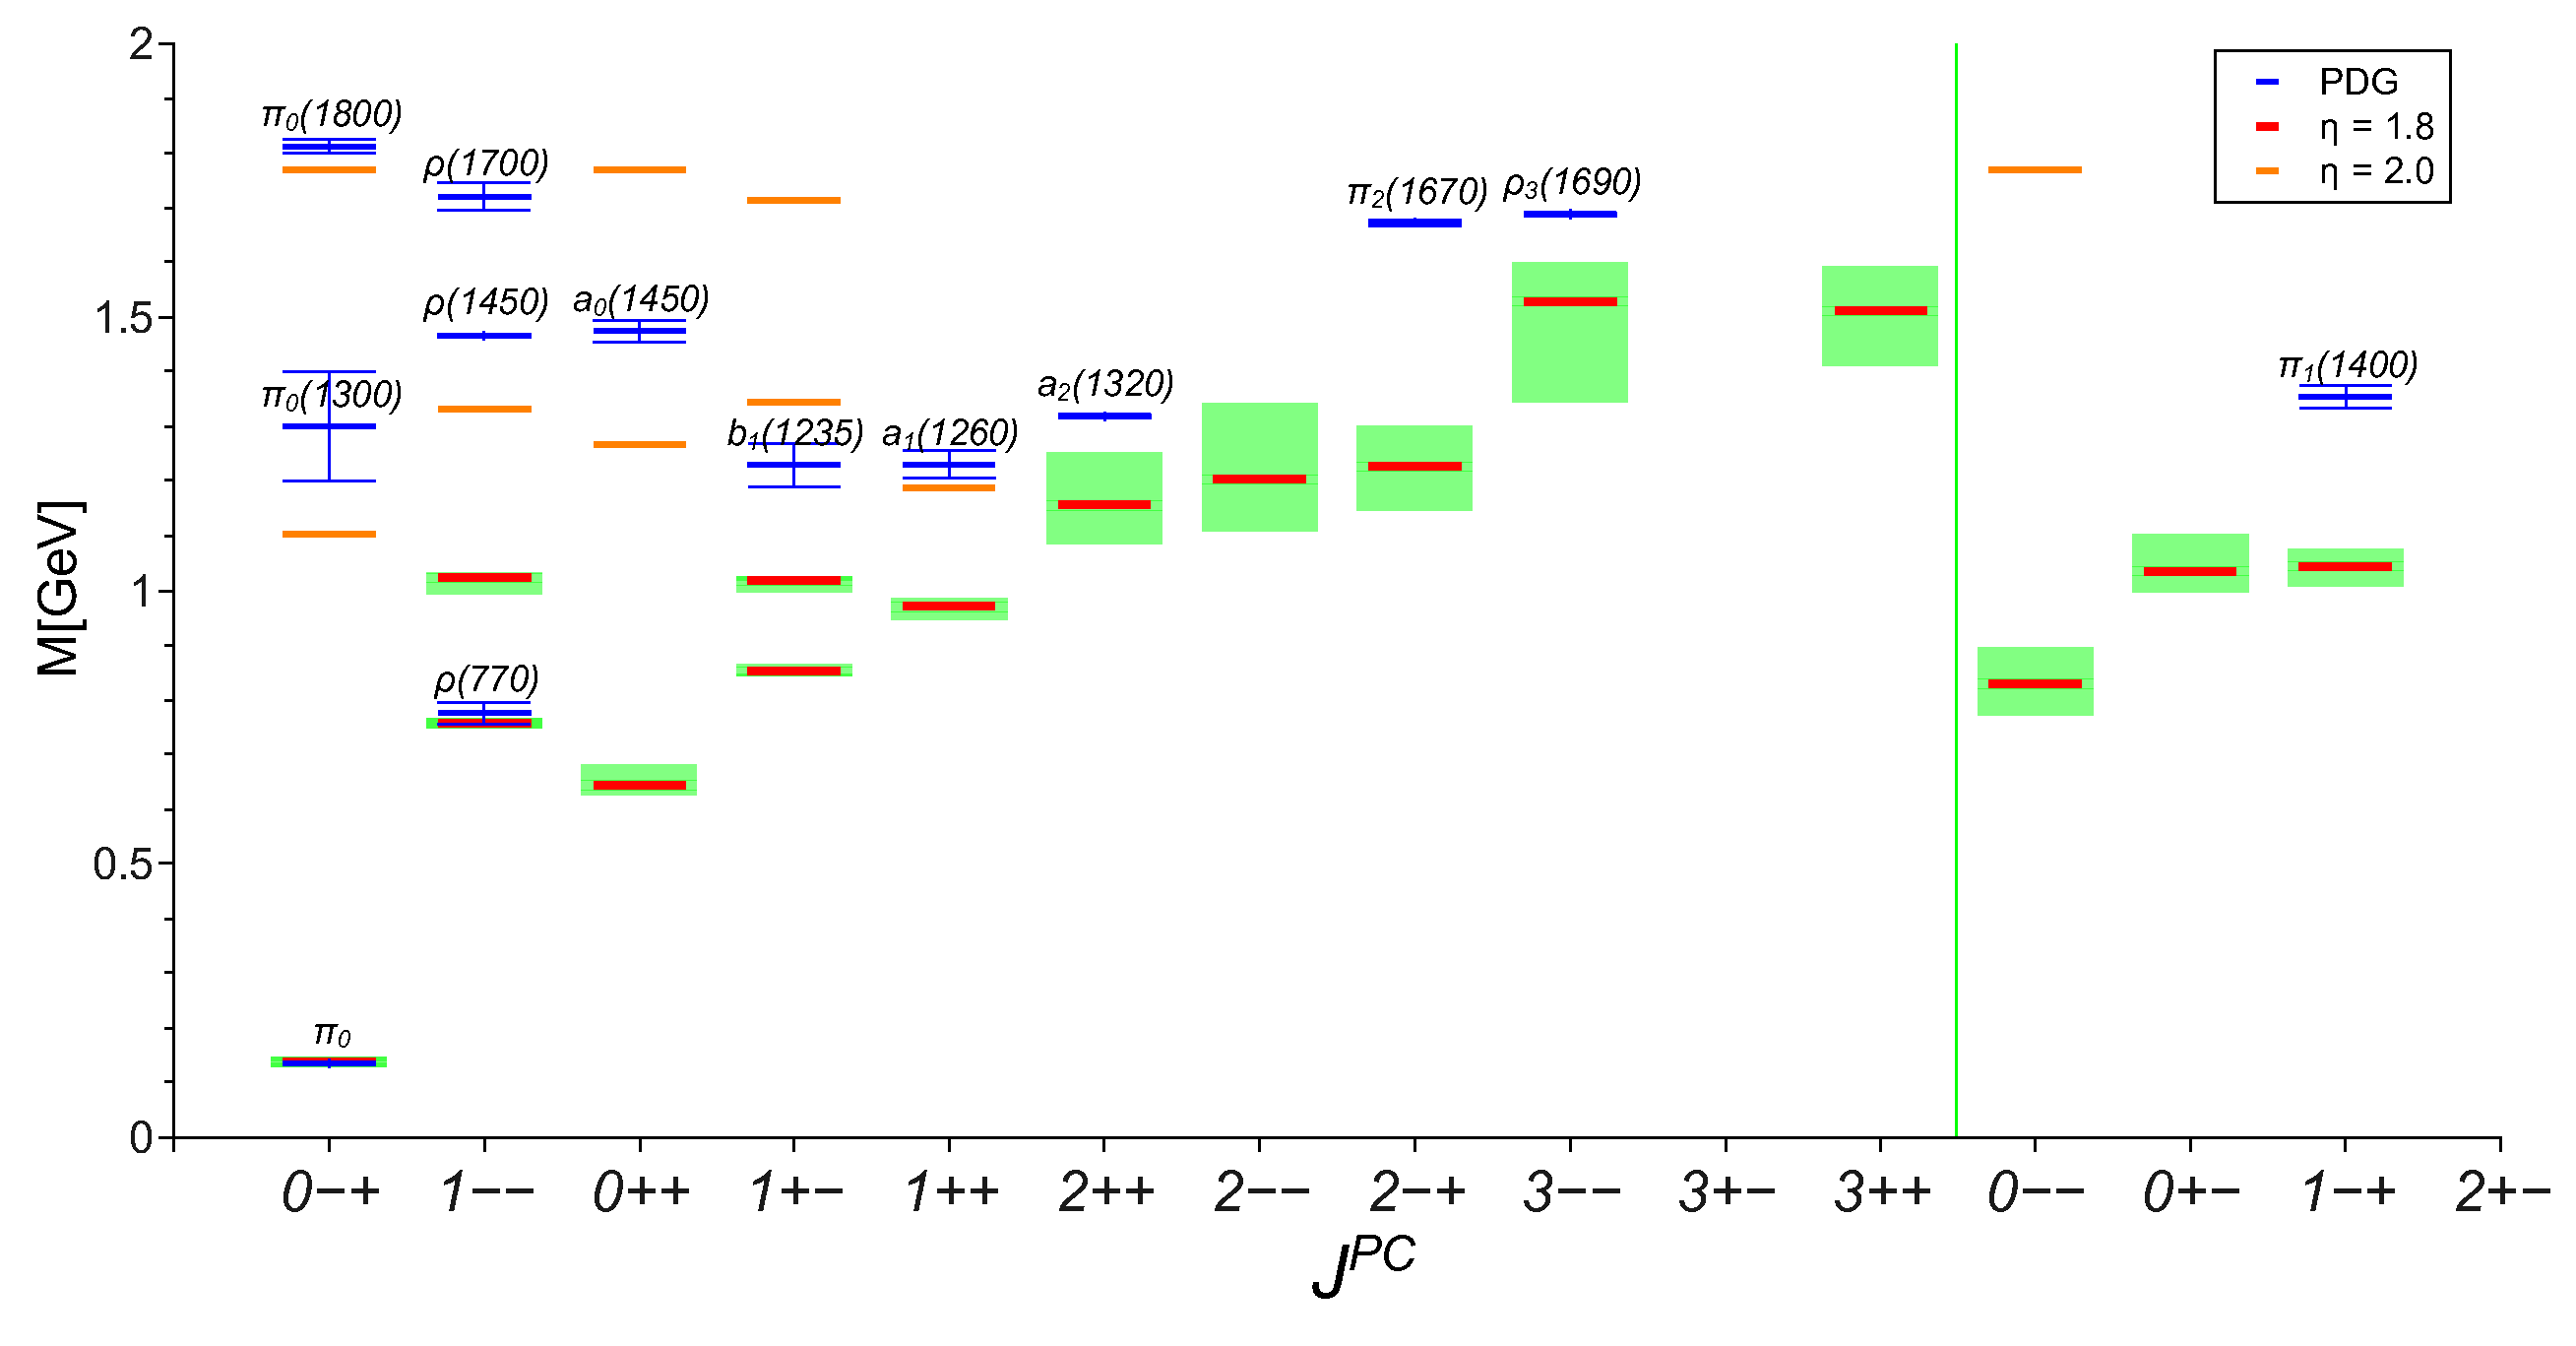
\includegraphics[width=0.999\textwidth]{figures/spectrum_nn}
\caption{\footnotesize The calculated $n\bar{n}$ spectrum, compared to the isovector mesons as measured in 
experiment. The green bands correspond to the 
variation $\eta=1.8\pm0.2$. Due to the structure of the propagator, in the case of $\eta=2.0$ more states are accessible; 
these are given by the single orange lines. The states to the right of the dividing line correspond to exotic quantum 
numbers.}\label{fig:spectrumnn}
\end{center}
\end{figure*}
In the RL approximation the interaction kernel admits no mixing between states. Furthermore we work in the isospin symmetric limit using equal current quark masses $m_u=m_d=0.0037$ GeV at a renormalization scale of $\mu = 19$ GeV. Thus, our calculated meson spectrum is degenerate in the isoscalar/isovector channel for $n=u,d$ quarks. Th explicit numbers can be found in the Appendix in Table \ref{tab:results}. In Fig.~\ref{fig:spectrumnn} we display the resulting spectrum for $n\bar{n}$ mesons, and compare with the isovector channel from experiment. The input up/down quark masses are fixed such that the experimental mass of the $\pi_0$ is reproduced. The resulting ground state mass in the vector channel is also in good agreement with experiment. This is not true, however, for the scalar and axialvector states as noted frequently before, see e.g. \cite{Watson:2004kd}. Here, the deficiency of the rainbow-ladder truncation is obvious and on the 20-40 \% level. In the scalar channel there is some evidence that the lowest lying nonet may not be identified as simple quark-antiquark states, but may be better described as tetraquarks, see {\it e.g.} \cite{Jaffe:1976ig,Giacosa:2006tf,Ebert:2008id,Parganlija:2012fy,Heupel:2012ua} and Refs. therein. Therefore we compare with the $a_0(1450)$, noting that in rainbow-ladder and without potential mixing with the scalar glueball state there is no hope to reproduce the experimental value. The situation is considerably better for the lowest lying tensor state \cite{Krassnigg:2010mh}, which for the upper value of the considered $\eta$-band is even on the 5 $\%$ level compared to the experimental value. While the other tensor states are again far off, at least where comparison with experiment is possible, the situation is again acceptable for the tensor meson with $J=3$ and $PC=\{--\}$. Its mass of $1528^{+71}_{-184}$~MeV compares well with both the isovector $\rho_3$ of mass $1688.8\pm2.1$~MeV (shown in the figure) and the isoscalar $\omega_3$ of mass $1667\pm4$~MeV with again a deviation on the 5 $\%$ level for the upper range of the $\eta$-band. In contrast, we find no bound state in the $J^{PC}=3^{+-}$-channel, whereas for the $J^{PC}=3^{++}$ state with mass $1510^{+81}_{-100}$~MeV there is no well established experimental counterpart.
\begin{figure*}[h]
\begin{center}
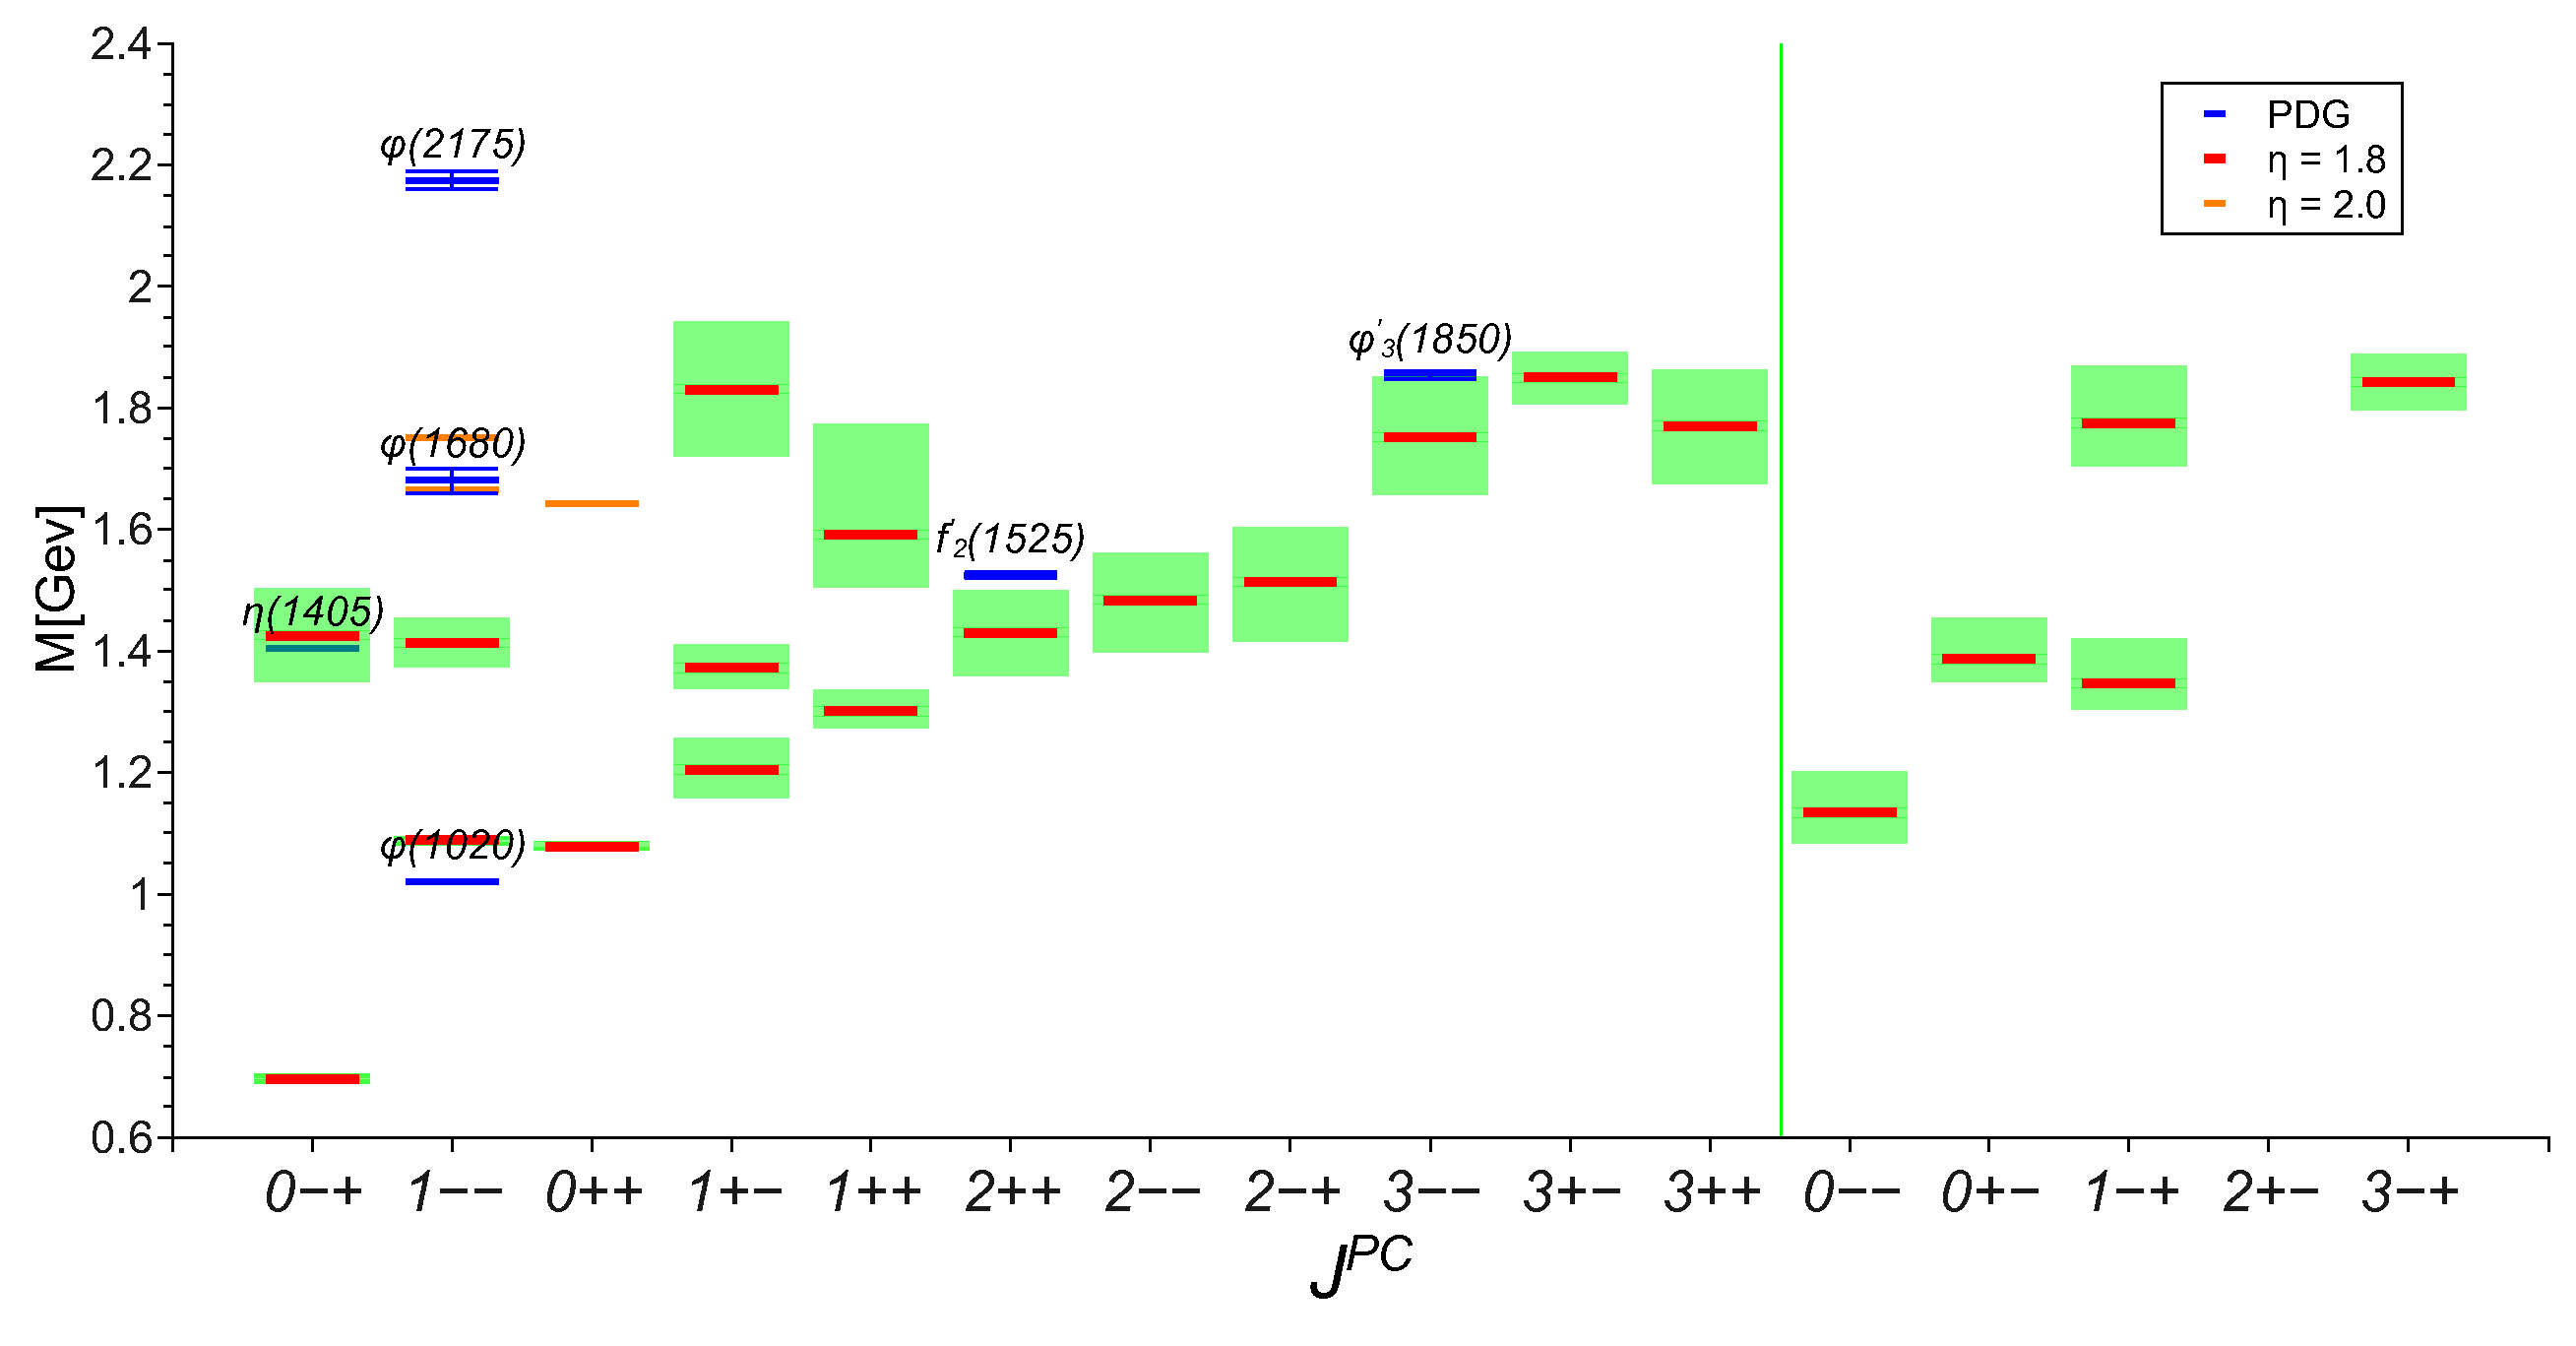
\includegraphics[width=0.999\textwidth]{figures/spectrum_ss}
\caption{ \footnotesize Calculated $s\bar{s}$ spectrum, compared to experiment. The green bands correspond to the 
variation $\eta=1.8\pm0.2$. Due to the structure of the propagator, in the case of $\eta=2.0$ more states are accessible; 
these are given by the single orange lines. The states to the right of the dividing line correspond to exotic quantum 
numbers.}\label{fig:spectrumss}
\end{center}
\end{figure*}
It is interesting to muse about the difference between the corresponding channels $J^{PC}=0^{-+},1^{--}$
as well as $J^{PC}=1^{--},2^{++},3^{--}$ in good agreement with experiment and the other channels that 
are further off, using notions of the (pseudo)-potentials in the quark model. In this language, what distinguishes these 
channels from the others is that the non-contact part of the spin-spin interaction 
is vanishing or small: for the hyperfine splitting between the pseudoscalar and vector 
channels the contact part of the spin-spin interaction is dominant, whereas for the $J^{PC}=2^{++},3^{--}$
states the spin-orbit forces prevail. For all other channels considered, there are sizeable 
contributions from the tensor part of the spin-spin interaction. Since these are the channels
that are off, we conclude, that the rainbow-ladder interaction roughly reproduces the size of
the contact part of the spin-spin interaction and the spin-orbit force, but materially overestimates
the binding in the tensor part of the spin-spin interaction. Note, that this conclusion is 
different than the one drawn in \cite{Qin:2011xq} based on only a subset of the states considered here.  
We come back to this discussion in section \ref{res:regge}.
\begin{figure*}[h]
\begin{center}
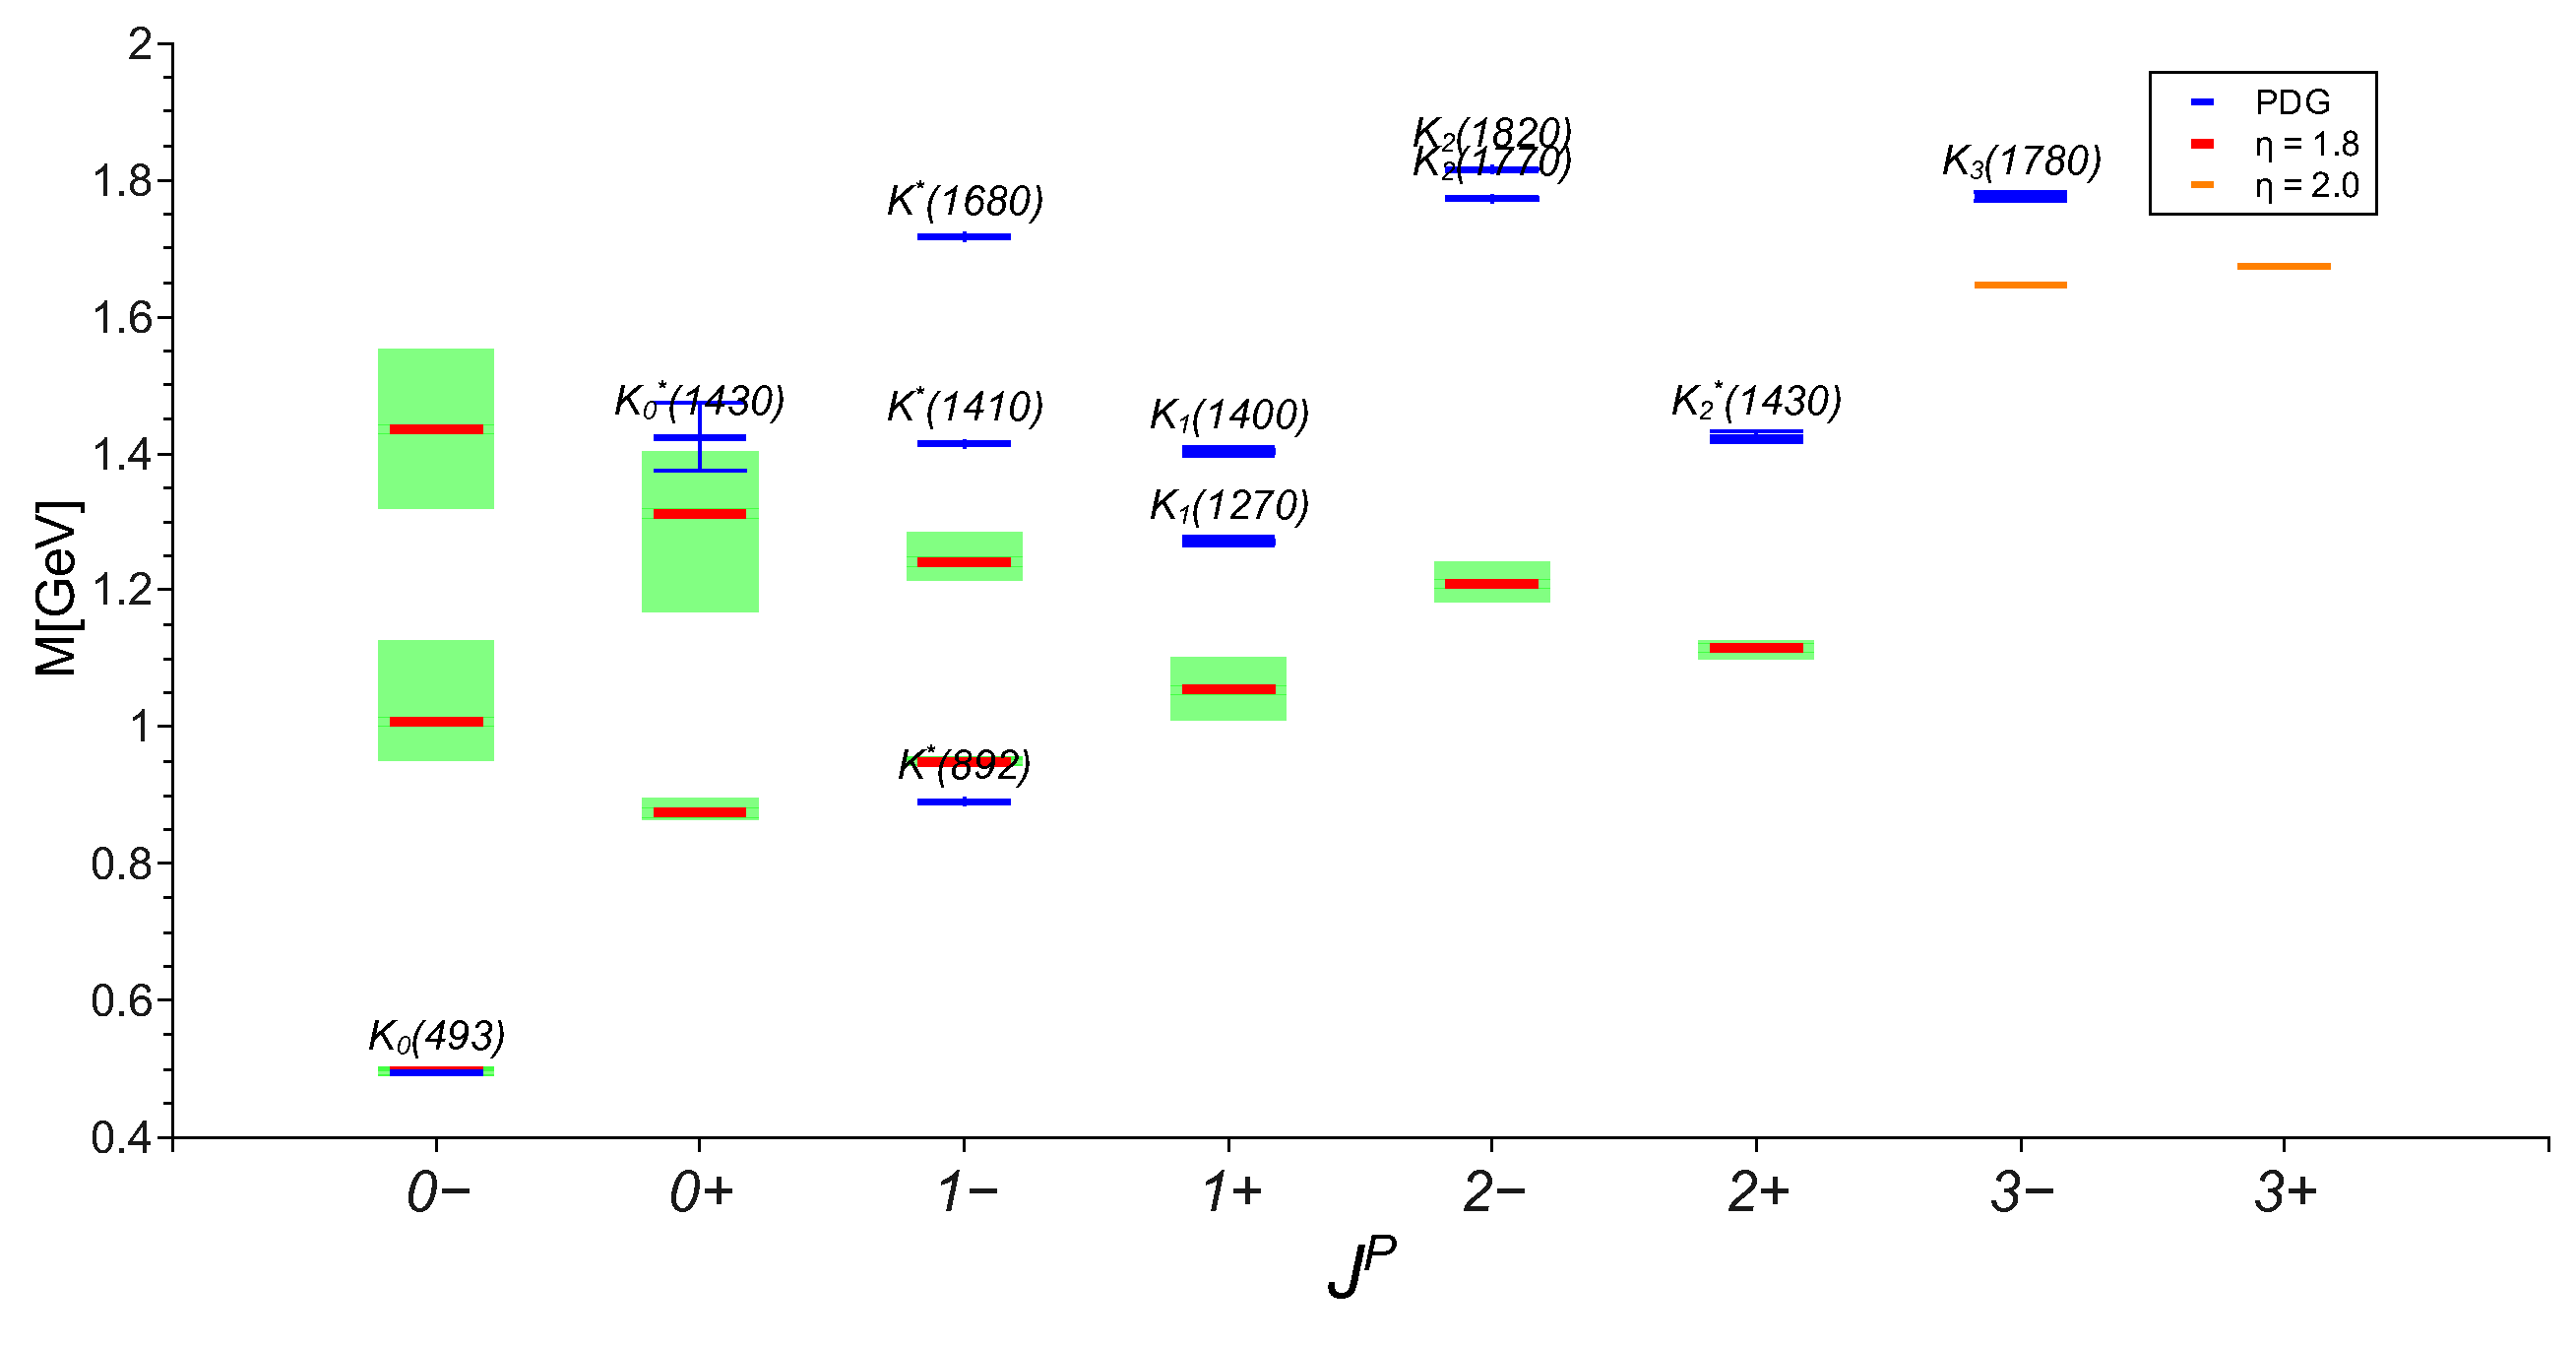
\includegraphics[width=0.999\textwidth]{figures/spectrum_ns}
\caption{\footnotesize Our calculated $n\bar{s}$ spectrum, compared to experiment. The green bands 
correspond to the variation $\eta=1.8\pm0.2$. Due to the structure of the propagator, in the case 
of $\eta=2.0$ more states are accessible; these are given by the single orange lines. The states 
to the right of the dividing line correspond to exotic quantum numbers.
 }\label{fig:spectrumns}
\end{center}
\end{figure*}
As for the exotic channels we find states for $J^{PC}=0^{--},0^{+-}$ with no experimentally established
counterpart, whereas our value for the $J^{PC}=1^{-+}$ is about 25 $\%$ lower than the $\pi_1(1400)$.
This finding is consistent with the ones in the axial-vector channels. In the exotic channels
with $J=2,3$ we do not find bound state.

Finally let us comment on the excited states. These are in general much too low \cite{Holl:2004fr}
in agreement with the general finding for the ground states. A variation of the $\eta$-value
in general does not improve this picture; also it is noteworthy that higher excited states only
appear for very specific values of $\eta$. This suggests a dependency of the excited states on 
the details of the momentum and tensor dependence of the quark-gluon interaction that needs to be explored 
in future work. \\

Next we discuss the $s\bar{s}$ spectrum given in the Appendix and displayed in Fig.~\ref{fig:spectrumss}.
Here the input value of the strange quark mass of $m_s(19 \,\mbox{GeV}) = 0.085$ GeV at the renormalization
point is determined from matching to the experimental value of the kaon discussed below.
First note that the pseudoscalar $s\bar{s}$-state is too light in this truncation since neither the 
effect of the $U_A(1)$ anomaly (see {\it e.g.} \cite{Alkofer:2008et} for a treatment of the anomaly
in the BSE formalism) nor flavor mixing with the $n\bar{n}$ states is considered. For the excited 
state in the pseudo-scalar channel the surprisingly excellent agreement with the $\eta(1405)$ extracted from
experiment may be accidental. In the vector channel, where mixing effects do not play a major role we
observe good agreement of our bound state mass with experiment. The same is true for the $J^{PC}=2^{++}$
and $J^{PC}=3^{--}$ channels, where the upper boundary of the $\eta$-band almost reproduces the
experimental values for the $f_2(1525)$ and the $\varphi_3(1850)$. Again, these are the channels
with dominating spin-orbit forces in the language of the potential models. In general, the pattern of
states in the $s\bar{s}$ spectrum is very similar to the one found for the $n\bar{n}$ mesons due
to the flavor independence of the underlying rainbow-ladder interaction model. \\

In the case of strange mesons, $n\bar{s}$, one is no longer able to assign either $C$ or $G$ 
parity to a state. Thus, here there are no states with explicitly exotic quantum numbers.

The spectrum, as calculated within the rainbow-ladder approximation, is given in Fig.~\ref{fig:spectrumns}. 
As already mentioned above, the strange quark mass is chosen such that the calculated $K^{0,\pm}$ 
is in agreement in experiment; the remaining spectrum is a result of the model.
While the vector ground state is in reasonable agreement with experiment, the remaining spectrum 
does not fare so well (as in the unflavored case).

Along with the usual $J=1$ and $J=2$ mesons, we find two states with $J=3$, one with positive 
and one with negative parity. For the latter, we have a mass of $1646.9$ (found for $\eta=2.0$ only) 
which compares well with the experimentally known $K_3^\star$ whose mass $1776\pm7$ is within $10\%$. 
The positive parity state is similar in mass, $1673.4$, but the putative $K_3$ has not been seen in 
experiment. 

The results strongly indicate that the $n\bar{s}$ system should be investigated in a beyond rainbow-ladder 
approximation, in order to find stronger agreement for the majority of low-lying states. In particular, the
$2^+$ channel is interesting since the experimentally observed states are considerably higher in mass than 
the calculated ones, in contrast to the findings discussed before in the flavor diagonal channels. On the
other hand, our numerical error in extracting the bound state masses is considerably higher in the
non-diagonal flavor case than in the diagonal one such that it is not clear whether the deficiency is in the
interaction or in our numerical procedure. This needs to be explored further.

%
%
%
%
%
\subsection*{Regge trajectories}\label{res:regge}
Finally, we present results for Regge trajectories in Fig.~\ref{fig:regge} for natural parity states. 
We only take into account trajectories with at least three states, which leaves the ground state isovector $n\bar{n}$ 
and isoscalar $s\bar{s}$ mesons with natural parity; for the corresponding excited states and the 
other channels we do not have enough bound states with $J=2,3$ to probe for trajectories. 
One immediately notes that, indeed, the sequence $J^{PC}=1^{--}, 2^{++}, 3^{--}$ forms an almost linear
trajectory in the $(M^2,J)$-plane. This is interesting, since we are working with a model that is
apparently \emph{not} related to a linear rising potential between light quarks. 

Thus, the conventional, naive but intuitive explanation for the formation of Regge-trajectories does not apply
in our framework. Nevertheless, we see an (approximate) $\rho$- and $\phi$-meson Regge trajectory 
for our results. The slope of the trajectory is easily extracted. With
\begin{equation}
M^2_X(J) = M^2_X(0) + \beta_X J
\end{equation} 
we find
\begin{eqnarray}
M^2_\rho(0) &=& -0.42 \,\,(-0.05)\,\, \mbox{GeV}^2 \nonumber\\
\beta_\rho &=& \,\,0.99 \,\,(0.62)\,\, \mbox{GeV}^2 \nonumber
\end{eqnarray}
and 
\begin{eqnarray}
M^2_\phi(0) &=& \,\,0.05 \,\,(0.36)\,\, \mbox{GeV}^2 \nonumber\\
 \beta_\phi &=& \,\,1.12 \,\,(0.78)\,\, \mbox{GeV}^2 \nonumber
\end{eqnarray}
for $X=\rho$ and $X=\phi$ respectively. The two numbers each correspond to the upper (lower)
end of the $\eta$-band of our results. Compared to recent studies of Regge trajectories
based on the $\rho$-meson, $\beta_\rho = 1.19 \pm 0.10$ GeV$^2$ \cite{Masjuan:2012gc} and 
$\beta_\rho = 1.11 \pm 0.01$ GeV$^2$ \cite{Londergan:2013dza}, our number for the slope at the
upper edge of the $\eta$-band is smaller by only about 
ten percent. Recalling that we need to employ an extrapolation procedure in the complex 
momentum plane to extract the bound state mass of the tensor states with an error margin 
of the order of 5-10 $\%$ the agreement is quite good.
\begin{figure}[h]
\begin{center}
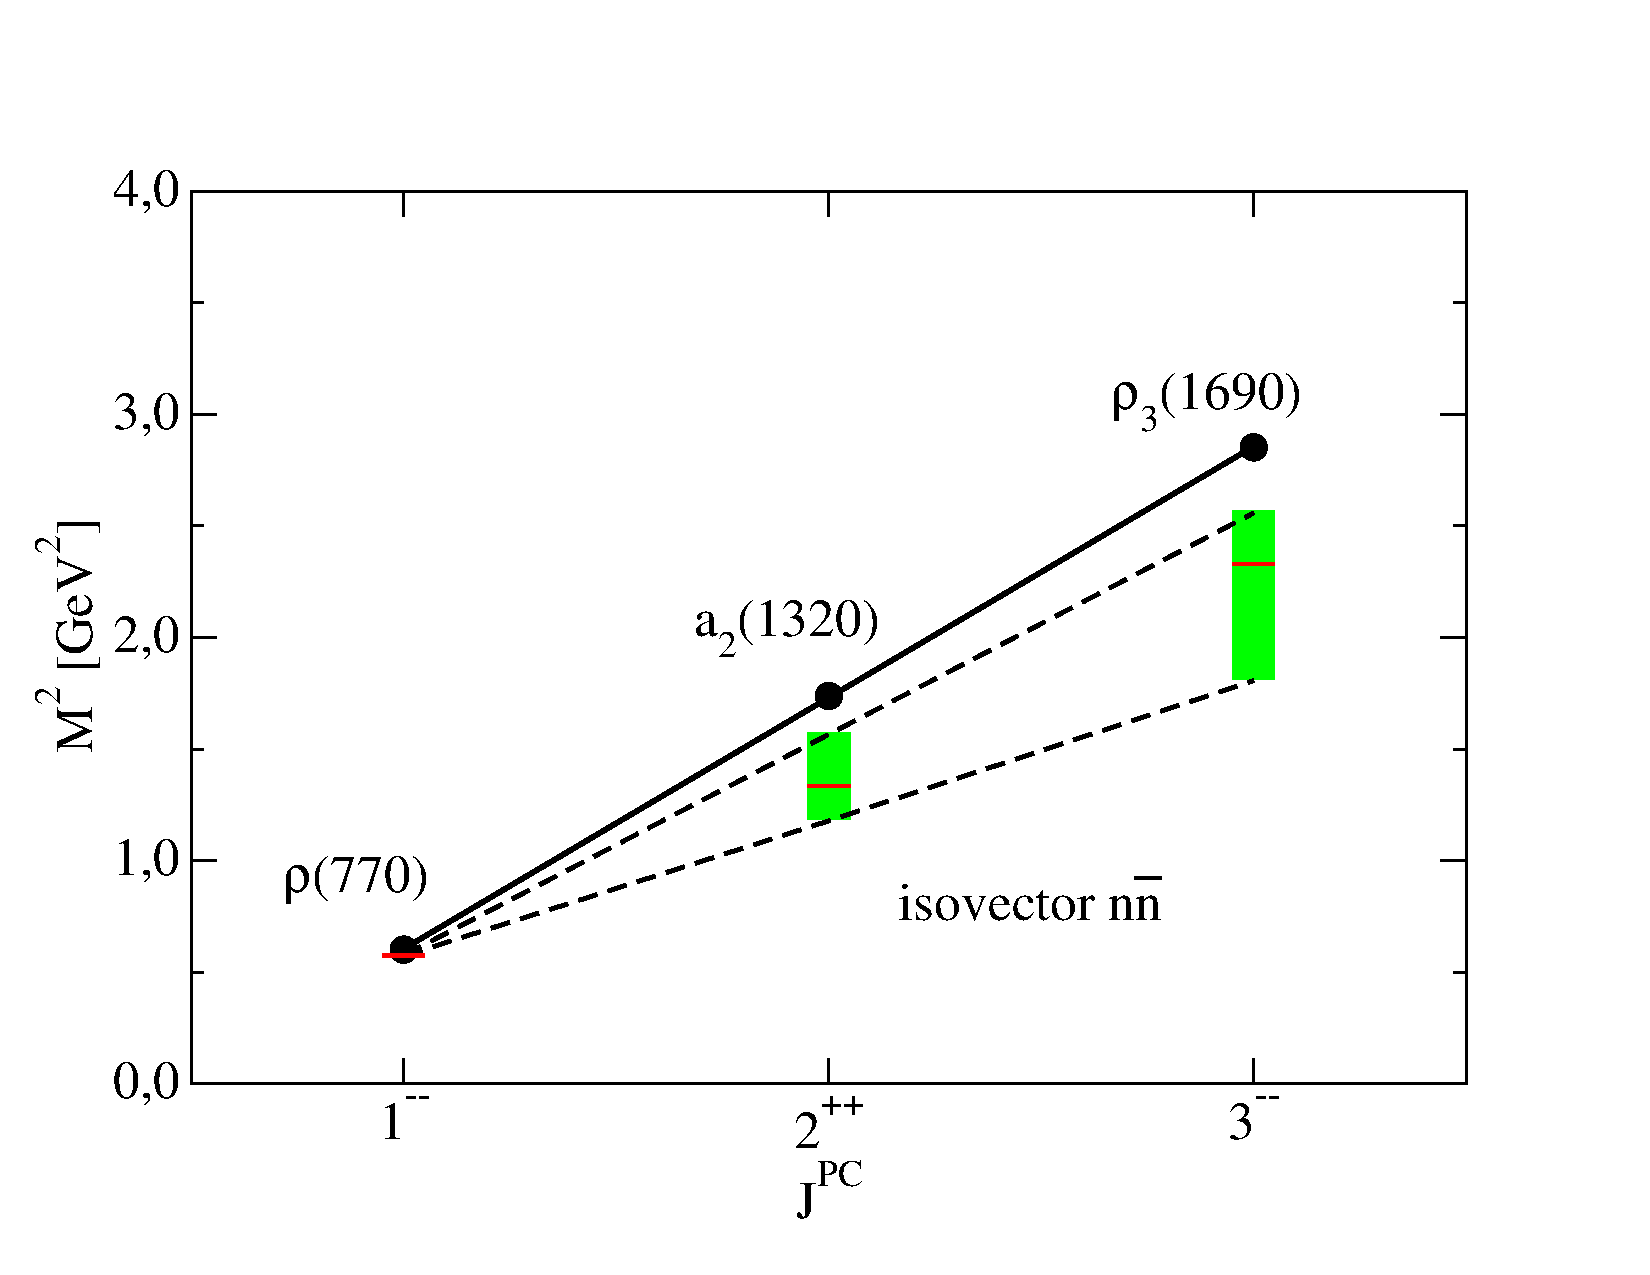
\includegraphics[width=0.49\textwidth]{figures/reggenn_v2}
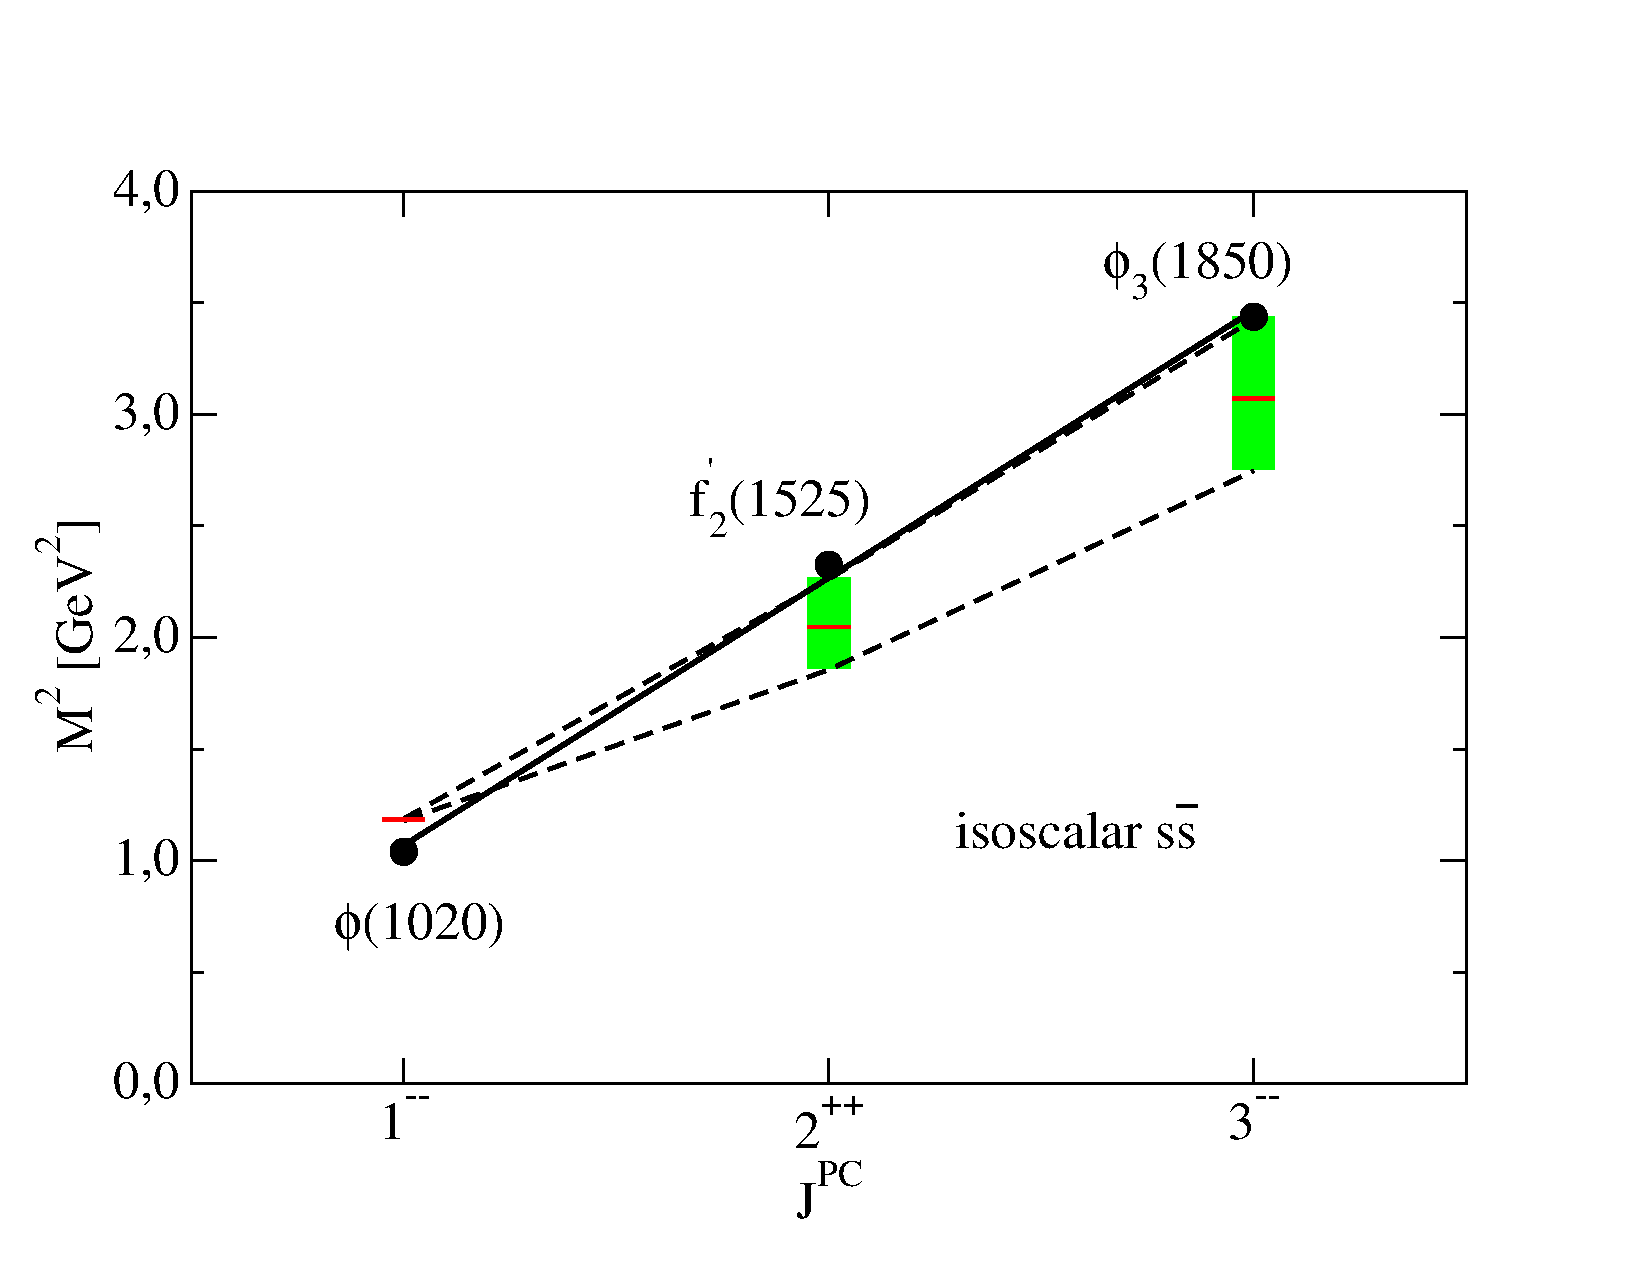
\includegraphics[width=0.49\textwidth]{figures/reggess_v2}
\caption{\small Regge trajectories for isovector $n\bar{n}$ (upper plot)
and isoscalar $s\bar{s}$ mesons (lower plot) with natural parity. 
Filled circles correspond to experimental data, while calculated values are given by the red marks
for $\eta = 1.8$ and the green bands for $\eta = 1.8 \pm 0.2$. The resulting Regge trajectories for 
the upper and lower end of the bands are displayed by the dashed lines. Not shown is the numerical
error of our mass extraction procedure, which is of the order of 5-10 $\%$ for the $J=2,3$ states.}\label{fig:regge}
\end{center}
\end{figure}
We have also checked for Regge trajectories in channels with unnatural parity and found an 
approximate linear trajectory also for the sequence $J^{PC}=1^{++}, 2^{--}, 3^{++}$ based 
on the $a_0$. Again, for the other channels and the excited states we find not enough bound 
states with $J=2,3$. From the discussion in the previous sections we furthermore expect, 
that the slopes and intercepts in these channels may be further off the experimentally extracted 
values, simply because the rainbow-ladder interaction is not good enough in these channels. 
Indeed for the $a_0$-trajectory we find $M^2_{a_0}(0) = 0.20\,\, \mbox{GeV}^2$ and
$\beta_{a_0} = 0.78 \,\,\mbox{GeV}^2$ for the upper edge of the $\eta$-band, which do not 
agree too well with {\it e.g.} the values found in Ref.~\cite{Ebert:2009ub}, 
$M^2_{a_0}(0) = -0.658 \pm 0.120\,\, \mbox{GeV}^2$ and
$\beta_{a_0} = 1.014 \pm 0.036 \,\,\mbox{GeV}^2$.
%
\begin{table*}[!th]
\renewcommand{\arraystretch}{1.3}
\begin{tabular}{c|ccc|ccc||c|ccc}
\hline
\hline
                            & \multicolumn{3}{c|}{$n\bar{n}   $}                                                         & \multicolumn{3}{c||}{$s\bar{s}$}                                           &          & \multicolumn{3}{c}{$n\bar{s}$}  \\
$J^{PC}$                    & $n=0$                                &   $n=1$                            &          $n=2$ & $n=0$                     &   $n=1$                   &          $n=2$    &  $J^P   $&  $n=0$    &$n=1$  & $n=2$ \\
\hline                                                                                                                                                                                                     
$0^{-+}$                    & $138.1^{+1.3}_{-0.6}$                &   $1103.0^\dag$                    &  $1770.1^\dag$ &  $696.3^{+2.4}_{-1.7}$    &  $1426.3_{-76.6}$         &                   &  \multirow{2}{*}{$0^-$}       &   \multirow{2}{*}{ $496.6^{+5.3}_{-0.9}$} &  \multirow{2}{*}{$1007.6^{+118.3}_{-\phantom{1}57.0}$ } & \multirow{2}{*}{$1435.9$} \\                                                                                                                                                                        
$0^{--}$                    & $828.8^{+66.9}_{-57.1}$              &                                    &                &  $1133.8^{+68.0}_{-50.8}$ &                           &                   &         &     & & \\
$0^{++}$                    & $643.6^{+17.6}_{-37.6}$              &   $1266.9^\dag$                    &  $1769.1^\dag$ &  $1079.4^{+1.7}_{-7.9}$   &  $1643.6^\dag$            &                   &  \multirow{2}{*}{$0^+$}       &  \multirow{2}{*}{ $874.5^{+10.0}_{-22.2}$ } &  \multirow{2}{*}{$1312.5^{+\phantom{1}90.3}_{-143.8}$} & \multirow{2}{*}{} \\                                                                                                                                                                        
$0^{+-}$                    & $1035.5^{+66.8}_{-38.8}$             &                                    &                &  $1386.7^{+68.8}_{-37.9}$ &                           &                   &         &     & & \\
\hline                                                                                                                                                                                                     
$1^{-+}$                    & $1043.9_{-37.0}$                     &                                    &                &  $1347.3^{+73.2}_{-43.7}$ &  $1870.1^{\ddag}$         &                   &  \multirow{2}{*}{$1^-$}       &   \multirow{2}{*}{$ 950.1^{+5.5}_{-1.6}$} &  \multirow{2}{*}{$1241.6^{+43.5}_{-27.9}$ } & \multirow{2}{*}{  } \\
$1^{--}$                    & $757.2^{+1.2}_{-0.6}$                & $1022.6^{+\phantom{1}9.2}_{-29.2}$ & $1331.9^\dag$  &  $1087.8^{+1.8}_{-2.2}$   &  $1413.1^{+38.8}_{-42.1}$ &   $1666.9^\dag$   &         &     & & \\                                                                                                                                                                       
$1^{++}$                    & $969.4^{+15.6}_{-23.9}$              & $1188.1^\dag$                      &                &  $1301.0^{+34.7}_{-28.5}$ &  $1591.9^{+181.2}$        &                   &  \multirow{2}{*}{$1^+$}       & \multirow{2}{*}{$1054.1^{+48.7}_{-44.8}$} &  \multirow{2}{*}{} & \multirow{2}{*}{} \\
$1^{+-}$                    & $852.1^{+13.6}_{-\phantom{1}5.2}$    & $1017.4^{+\phantom{1}0.6}_{-21.4}$ & $1345.2^\dag$  &  $1205.1^{+51.8}_{-46.6}$ &  $1372.0^{+34.4}_{-39.5}$ &   $1831.6^\dag$   &         &     & & \\
\hline                                                                                                                                                                                                     
$2^{-+}$                    & $1226.5^{+73.9}_{-80.0}$             &                                    &                &  $1513.5^{+90.5}_{-85.0}$ &                           &                   &  \multirow{2}{*}{$2^-$}       &  \multirow{2}{*}{ $1116.2^{+10.9}_{-17.2}$ } &  \multirow{2}{*}{} & \multirow{2}{*}{} \\
$2^{--}$                    & $1202.6^{+140.0}_{-\phantom{1}94.3}$ &                                    &                &  $1484.7^{+76.0}_{-86.0}$ &                           &                   &         &     & & \\
$2^{++}$                    & $1154.8^{+96.5}_{-69.3}$             &                                    &                &  $1431.4^{+72.4}_{-69.3}$ &                           &                   &  \multirow{2}{*}{$2^+$}       &  \multirow{2}{*}{$1209.4^{+32.3}_{-26.6}$} &  \multirow{2}{*}{} & \multirow{2}{*}{} \\
$2^{+-}$                    &                                      &                                    &                &                           &                           &                   &         &     & & \\
\hline                                                                                                                                                                                                     
$3^{-+}$                    &                                      &                                    &                &  $1842.5_{-46.6}$         &                           &                   &  \multirow{2}{*}{$3^-$}       & \multirow{2}{*}{ $1646.9^\dag$ }  &  \multirow{2}{*}{} & \multirow{2}{*}{} \\
$3^{--}$                    & $1528.3^{+\phantom{1}71.2}_{-184.2}$ &                                    &                &  $1751.7^{+99.2}_{-94.3}$ &                           &                   &         &     & & \\
$3^{++}$                    & $1510.5^{+\phantom{1}81.6}_{-100.3}$ &                                    &                &  $1770.9^{+91.4}_{-96.1}$ &                           &                   &  \multirow{2}{*}{$3^+$}       & \multirow{2}{*}{ $1673.4^\dag$  } &  \multirow{2}{*}{} & \multirow{2}{*}{} \\
$3^{+-}$                    &  									&                                    &                &  $1849.4_{-43.6}$  &                           &                   &         &     & & \\                                                                                                                                                                      
\hline
\hline
\end{tabular}
\caption{Mass spectrum in MeV for isospin degenerate $n\bar{n}$, isoscalar $s\bar{s}$, and $I=1/2$ $n\bar{s}$ bound-states. The rainbow-ladder result corresponds to $\eta=1.8\pm0.2$, with the 
superscript ${}^\dag$ (${}^\ddag$) indicating $\eta=2.0$ ($\eta=1.6$) only.}\label{tab:results}
\end{table*}
%
%
%
%
%
%
\\

We presented the covariant decomposition of quark-antiquark bound states for $J\le3$, 
following~\cite{Joos:1962qq,Weinberg:1964cn} and \cite{Zemach:1968zz}. Within the 
rainbow-ladder truncations using a well-established effective interaction we calculated 
the spectrum of light unflavored and strange mesons. Comparison with experiment highlights 
the need to explore truncations beyond that of rainbow-ladder; in particular the effects 
of mixing as well as the introduction of a flavor dependent interaction are needed.
In the language of potentials for the spin-spin and spin-orbit forces we find 
sizable deviations in all channels, where the tensor part of the spin-spin interaction is important.
These are in particular the scalar and axialvector channels. On the other hand, the results
are quantitatively reliable on the five percent level (at least for the upper end of the 
checked $\eta$-band of the interaction parameter) for channels where only the contact part
of the spin-spin interaction plays a role, {\it i.e.} the hyperfine splitting of the
$S$-states, and channels dominated by the spin-orbit force, {\it i.e.} $J^{PC}= 2^{++}, 3^{--}$.
As a consequence, we find that the ground state Regge trajectory based on the $\rho$-meson
agrees with extractions from experiment on the ten percent level. Since our approach is
{\it not} based on a linear rising potential between light quarks, it is interesting that 
we see approximate Regge trajectories in the first place. This sheds some doubt on the
intuitive but naive interpretation of Regge-behavior as originating from color flux tubes.
The alternative mechanism at work in our framework needs to be explored further. 
Future work will also focus on the accessibility of excited states through a proper
treatment of the quark propagator poles in both the quark DSE and meson BSE, in 
addition to an exploration of the heavy-heavy and heavy-light meson spectrum.

\section{Heavy quark section}
With the spectacular success of Belle, Babar, BES and the LHC 
experiments and their discovery of an ever increasing and
largely unexplained number of XYZ-states, hadron spectroscopy 
in the heavy quark region became a fascinating topic in the 
past years. Many of the newly discovered states are surprisingly 
narrow, with some of these states electrically charged and
therefore not accounted for by the conventional quark model picture 
of quark-antiquark meson bound states.
Certainly, the potential of these states to guide us in our
understanding of the underlying physics of the strong interaction
is enormous, as detailed e.g. in Refs.~\cite{Brambilla:2010cs,
Pakhlova:2010zza,JohanMesschendorpfortheBESIII:2013vla,Bodwin:2013nua} 
and references therein.

From a theoretical QCD perspective charmonia (and, to a perhaps lesser 
degree, bottomonia) are extremely interesting since they combine effects 
of non-perturbative QCD with perturbative concepts in the heavy quark 
regime. In general, the charm quark is not heavy enough to be considered 
as non-relativistic. Thus especially excited states in the charmonium spectrum 
have to be considered in a framework that is genuinely relativistic or, 
at least, incorporates relativistic corrections. Model calculations in 
terms of relativistic quasipotentials reproduce many features of the spectrum
\cite{Godfrey:1985xj,Ebert:2002pp,Ebert:2011jc,LlanesEstrada:2011kc} and provide important
guidance on the structure of the spectrum. However, in order to gain a more 
systematic understanding of the underlying physics of the strong 
interaction it is mandatory to employ approaches that are directly rooted 
within QCD. At least two different strategies have been employed in this 
direction. On the one hand, lattice gauge theory as well as non-relativistic 
QCD (NRQCD) and potential NRQCD have made substantial progress in determining 
the details of the heavy quark potential from QCD~\cite{Brambilla:2004jw,Koma:2006si}. 

On the other hand, the heavy quarkonia states can be directly calculated 
from the underlying QCD Lagrangian without the need to resort to expansions 
in terms of quark velocities or heavy quark masses. Such approaches have the
obvious advantage that the heavy and the light quark sectors can be treated 
in the same framework. In the charmonium sector, lattice gauge theory has made 
an ever increasing effort to determine the spectrum of ground and excited states
as well as exotics in dynamical calculations, see e.g. 
\cite{Namekawa:2011wt,Bali:2011rd,Liu:2012ze,Moir:2013ub,Kalinowski:2013wsa}
and references therein as well as \cite{Mohler:2012gn,Prelovsek:2013cta} for short reviews.

An alternative approach based on QCD is the relativistic functional framework 
employing the Dyson-Schwinger and Bethe-Salpeter equations. Within the
rainbow-ladder approximation first studies of the quarkonium 
spectrum~\cite{Bhagwat:2006pu,Blank:2011ha,Hilger:2014nma,Popovici:2014pha} 
as well as exotic states like tetraquarks~\cite{Heupel:2012ua} 
in the heavy quark region have been performed, accompanied by 
systematic studies in the limit of static quarks~\cite{Popovici:2010mb,Popovici:2011yz,Popovici:2014usa}.

In this work we refine and extend these calculations in two directions. On 
the one hand we include states with higher angular momentum up to $J=3$.
On the other hand we perform a systematic study of the influence of 
details in the momentum dependence of the underlying effective running
coupling on the spectrum of ground and excited states in these channels.
We extend our analysis of~\cite{Fischer:2014xha} to the heavy $\bar{c}c$, $\bar{b}b$ 
and $\bar{b}c$ mesons. In the process, we generalize the frequently used Maris-Tandy 
interaction in order to explore the impact of the shape of the interaction, with 
an emphasis on the resultant splitting between different meson channels and their
excited states. 

The paper is organized as follows. In section~\ref{sec:framework} we summarize 
the framework of the DSE and BSEs, together with a discussion of the rainbow-ladder 
interaction employed. Our results are presented and discussed in section~\ref{sec:results}. 
We conclude in section~\ref{sec:conclusions}.

\subsection*{Charmonia}\label{sec:charm}

%
%
%
%
%
%
We start our study with what we term the vanilla Maris-Tandy interaction,
i.e. we keep the scale $\Lambda=0.72$ from the light meson sector and
explore the dependence of the spectrum on $\eta$. Furthermore, for the
polynomial $\mathcal{P}(x)$ in Eq.~(\ref{eqn:generalmaristandy2}) we 
employ the Maris-Tandy form ($a_2 = 1$, remaining $a_i =0$).
This original form of the Maris-Tandy interaction has been employed in the
heavy meson sector already in Ref.~\cite{Blank:2011ha}. However, there a general
fit to the ground states in several channels has been performed with the idea 
to minimise a general cost function. Here we employ a different strategy.
We utilise an observation made in~\cite{Fischer:2014xha}, namely that the channels 
$1^{--}, 2^{++},3^{--}$ etc. are particularly well represented in the 
rainbow-ladder framework. Within the realms of potential quark models these
states share the property that the spin-spin tensor forces do not play an 
important role. Since these states are well represented in the vanilla
Maris-Tandy (MT) interaction in the light meson sector, we first concentrate
on the ground and first excited states in the $1^{--}$ and $2^{++}$-channels
and explore the variation of the corresponding masses with the charm quark
mass and the $\eta$-parameter in the MT-interaction. We obtained good
agreement with experiment using a charm quark mass of 
$m(19 \,\mbox{GeV}) = 0.870 \,\mbox{GeV}$ and a value $\eta=1.157$.
\begin{figure*}[h]
  \begin{center}
  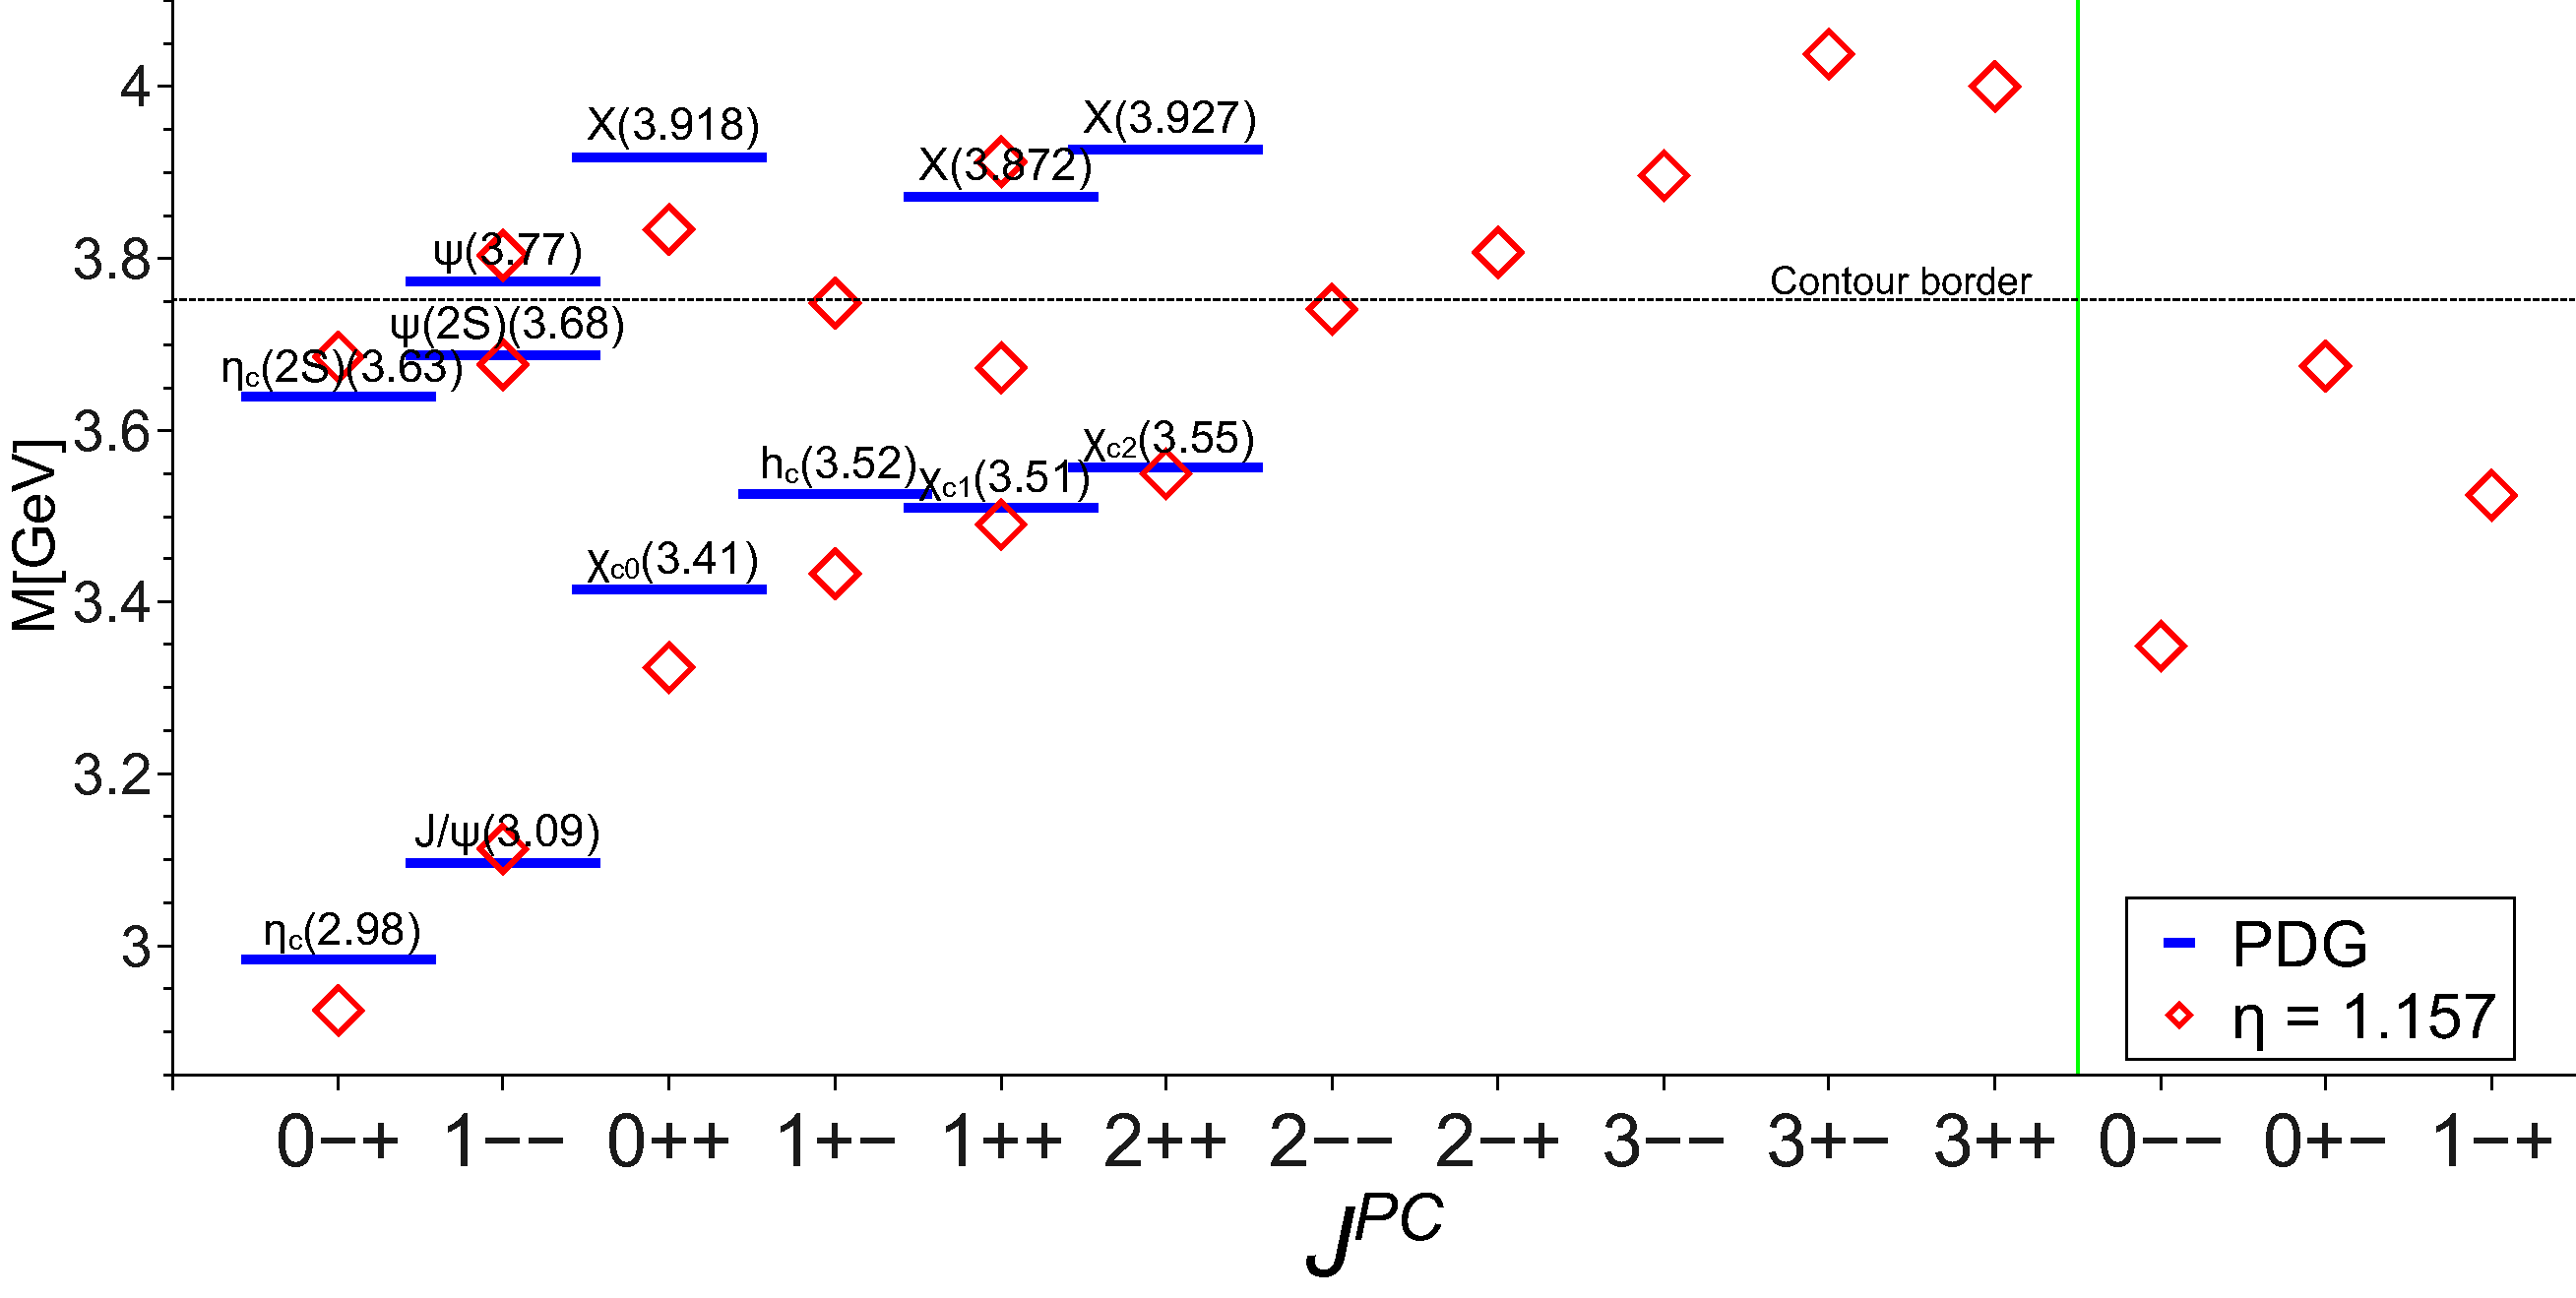
\includegraphics[width=0.999\textwidth]{figures/spectrum_cc}
  \caption{Spectrum of ground and excited charmonium states for the vanilla MT-rainbow-ladder interaction.}
  \label{fig:charm}
  \end{center}
\end{figure*}
Our results for all presently available channels are shown in Fig.~\ref{fig:charm},
the explicit values are all collected in Tab.~\ref{tab:results} at the end of the results section.
Since we have fixed the two input parameters with the $J/\Psi$ and $X_{c2}$ ground 
state, all other states can be viewed as model predictions. In the pseudoscalar channel
we find a mass of the $\eta_c$ which is slightly too low, but still within 3 \% of 
the experimental value. In the language of potential models, this may indicate an 
overestimation of the spin-spin contact term in the effective interaction. Very good 
agreement with experiment is obtained for the ground state in the $1_{++}$-channel, 
whereas the masses of
the scalar $0^{++}$ and the axialvector $1^{+-}$ ground states are further 
off but still within five percent of the experimental value. Similar results have
been obtained already in Ref.~\cite{Blank:2011ha,Hilger:2014nma}. The new element here is the
calculation of states with $J=3$ and the excited states. In Ref.~\cite{Fischer:2014xha}
we already observed in the light quark sector, that the rainbow-ladder interaction
is well suited to reproduce states in the sequence $1^{--}, 2^{++}, 3^{--},...$, which
are located on the same Regge-trajectory. We therefore expect our 
prediction for the mass of the $3^{--}$-state of 
%
\begin{align}
%
  m_{3^{--}}= 3896 \,\mbox{GeV}
%
\end{align}
%
to be accurate with an error below 1~\% due to uncertainties in the interaction.
Since this state is a ground state still close to the boundary of calculable states 
(the dashed line in the plot) it is not subject to a large extrapolation error. We 
therefore expect our prediction for the mass of this state to be quite robust, with 
an overall error on the 3~\% level. Within errors, this agrees with the quark model 
prediction \cite{Ebert:2011jc} and the lattice QCD results \cite{Bali:2011rd,Liu:2012ze}.
For the other tensor ground states with $J=2$ and $J=3$ we expect much less accurate 
predictions, perhaps on the 5-10~\% level. 

Similar to the light quark sector \cite{Fischer:2014xha} we also find, that the 
sequence $1^{--}, 2^{++}, 3^{--}$ lies on a Regge-trajectory with an accuracy that is
even better than in the potential model of Ref.~\cite{Ebert:2011jc}. 
For $J = \alpha M^2 + \alpha_0$ we find $\alpha = 0.36$ and $\alpha_0 = -2.55$, which 
is also somewhat steeper than the result of \cite{Ebert:2011jc}. For the heavy quark 
sector this confirms a result found in Ref.~\cite{Fischer:2014xha} for light quarks,
that Regge-type behaviour in the spectrum may be found without any direct connection 
to an underlying string-picture.

We also calculated the masses of ground states with exotic quantum numbers that cannot 
be accounted for as $q\bar{q}$-states in quark models. Our results are displayed in 
Fig.~\ref{fig:charm}. Note that within a genuinely relativistic framework such as 
lattice QCD or the functional approach used here, there is no problem representing these 
states with bilinear operators. Therefore they naturally appear also in the 
$q\bar{q}$-spectrum. Of course, it is then an open question, whether sizeable admixtures 
from states with a different quark content than $q\bar{q}$ (captured only in appropriate 
extensions of the quark-gluon interaction beyond rainbow-ladder) do exist. Furthermore,
even within the $q\bar{q}$-picture large corrections beyond rainbow-ladder may occur.
Because of these possibilities our calculated masses should be regarded with a lot of 
caution. 

For the excited states we observe very good agreement in the vector channel: our
value for the mass of the $\Psi(2S)$ is very close to the experimental one, and even
the next radial excitation is nicely represented. In the pseudoscalar channel the 
splitting between the ground and the excited state is slightly too large, making the 
agreement of the $(2S)$-state with experiment even better than for the ground state
$\eta_c$. It is interesting to observe that the resulting fine structure splitting of 
the ground and excited states show a qualitatively difference when compared with 
experiment: whereas the ground state splitting is too large the splitting in the 
excited state is too low. Such an uncorrelated behaviour of the two splittings has
also been observed in lattice QCD \cite{Bali:2011rd}.

In the `good' tensor channel $2^{++}$ potential excited states like
the $X(3927)$ are not reproduced in our framework. There is a considerable uncertainly 
due to the extrapolation procedure needed in this mass region, which is enhanced for
excited states. Taking our result at face value, however, the current model would disregard 
the notion of the $X(3927)$ to be an ordinary meson state.

From an experimental point of view, the $1^{++}$-channel is perhaps the most interesting
one. There the famous $X(3872)$-state awaits its identification as a meson-molecule,
a tetraquark, or an ordinary quark-antiquark bound state. The literature on this
subject is enormous, therefore we point the reader only to Ref.~\cite{Bodwin:2013nua} 
for a first overview. The interesting question in this context is, whether a description
on a quark-antiquark basis is possible at all for the $X(3872)$. In the present
rainbow-ladder model we find an excited state in the $1^{++}$-channel at 
$m = 3672 \,\mbox{MeV}$ that cannot be accounted for by experiment. A second excitation 
is found at $m = 3912 \,\mbox{MeV}$, close to the quark model prediction for the first
excited state. In principle, it could be that the lower state of the two is spurious.
However, since we find no trace in our numerics that this is the case we disregard this
notion for the moment. It follows then, that the present form of the rainbow-ladder 
interaction is not sufficient to describe the splitting between ground and excited states
in this channel. A similar conclusion may be drawn for the other axialvector channel.
We therefore expect sizeable corrections when interactions beyond the 
rainbow-ladder approximation are taken into account.\footnote{In addition, these states are above 
the $D\bar{D}$-threshold, where coupled channel effects may play an important role.}
This is the subject of future work. 
Here, as a first
step in this direction, we would like to explore the extent to which the rainbow-ladder 
interaction can be modified to increase the mass of the first excited $1^{++}$-state found 
in our model, without destroying the properties of the spectrum in the other channels. 
To this end we systematically explore the variations of the spectrum once we go away 
from the simple shape of the effective coupling Eq.~(\ref{eqn:generalmaristandy}) with 
polynomial $\mathcal{P}(x) = x^2$, i.e. $a_2=1$ and all other $a_i=0$ in 
Eq.~(\ref{eqn:polinomMT}). This is the subject of the next two subsections.
   
%
%
%
%

%
%
%
\subsection*{Bottomonia}\label{sec:bottom}

Our results for the spectrum of bottomonia are shown in Fig.~\ref{fig:bottom}. Compared to
the charmonium spectrum in Fig.~\ref{fig:charm} we had to change the shape of the interaction
by adjusting the $\eta$-parameter from $\eta=1.157$ for the charm-case to $\eta=1.357$ 
for the bottom quarks. This reflects part of the underlying flavour dependence of the quark-gluon 
interaction as noted in Ref.~\cite{Williams:2014iea}. Our corresponding mass of the bottom quark
is $m(19 \,\mbox{GeV})=3.790 \,\mbox{GeV}$. The resulting spectrum of ground and excited states, 
however, has similar features when compared with experimental values as the charmonium one. 
Once again, the $0^{-+}$, $1^{--}$ and $2^{++}$ ground states are well represented. The necessary
extrapolation needed for the $2^{++}$ is still under control, since the state is not too far above
the limit where everything can be calculated (the dashed line in the plot). Surprisingly good is
also the negative parity tensor state, although the extrapolation procedure in this
mass region must be considered with a little more caution. The ground states
in the scalar and axial vector channels are further off their experimental counterparts,
although still within the 1 \% deviation margin. Thus overall, the ground state spectrum
of bottomonia is well represented in the rainbow-ladder approximation of the BSEs.
Provided the good agreement in the $2^{--}$-channel can be seen as an indication that 
extrapolation even in this mass region works well, we can regard the masses of the 
further tensor states with $J=2$ and $J=3$ as more or less solid predictions 
on the level of one percent. Compared to the quark-model predictions of \cite{Ebert:2011jc}
we find only slight deviations of the order of 30-70 MeV for the $2^{-+}$ and the states 
with $J=3$.
%
\begin{figure*}[h]
  \begin{center}
    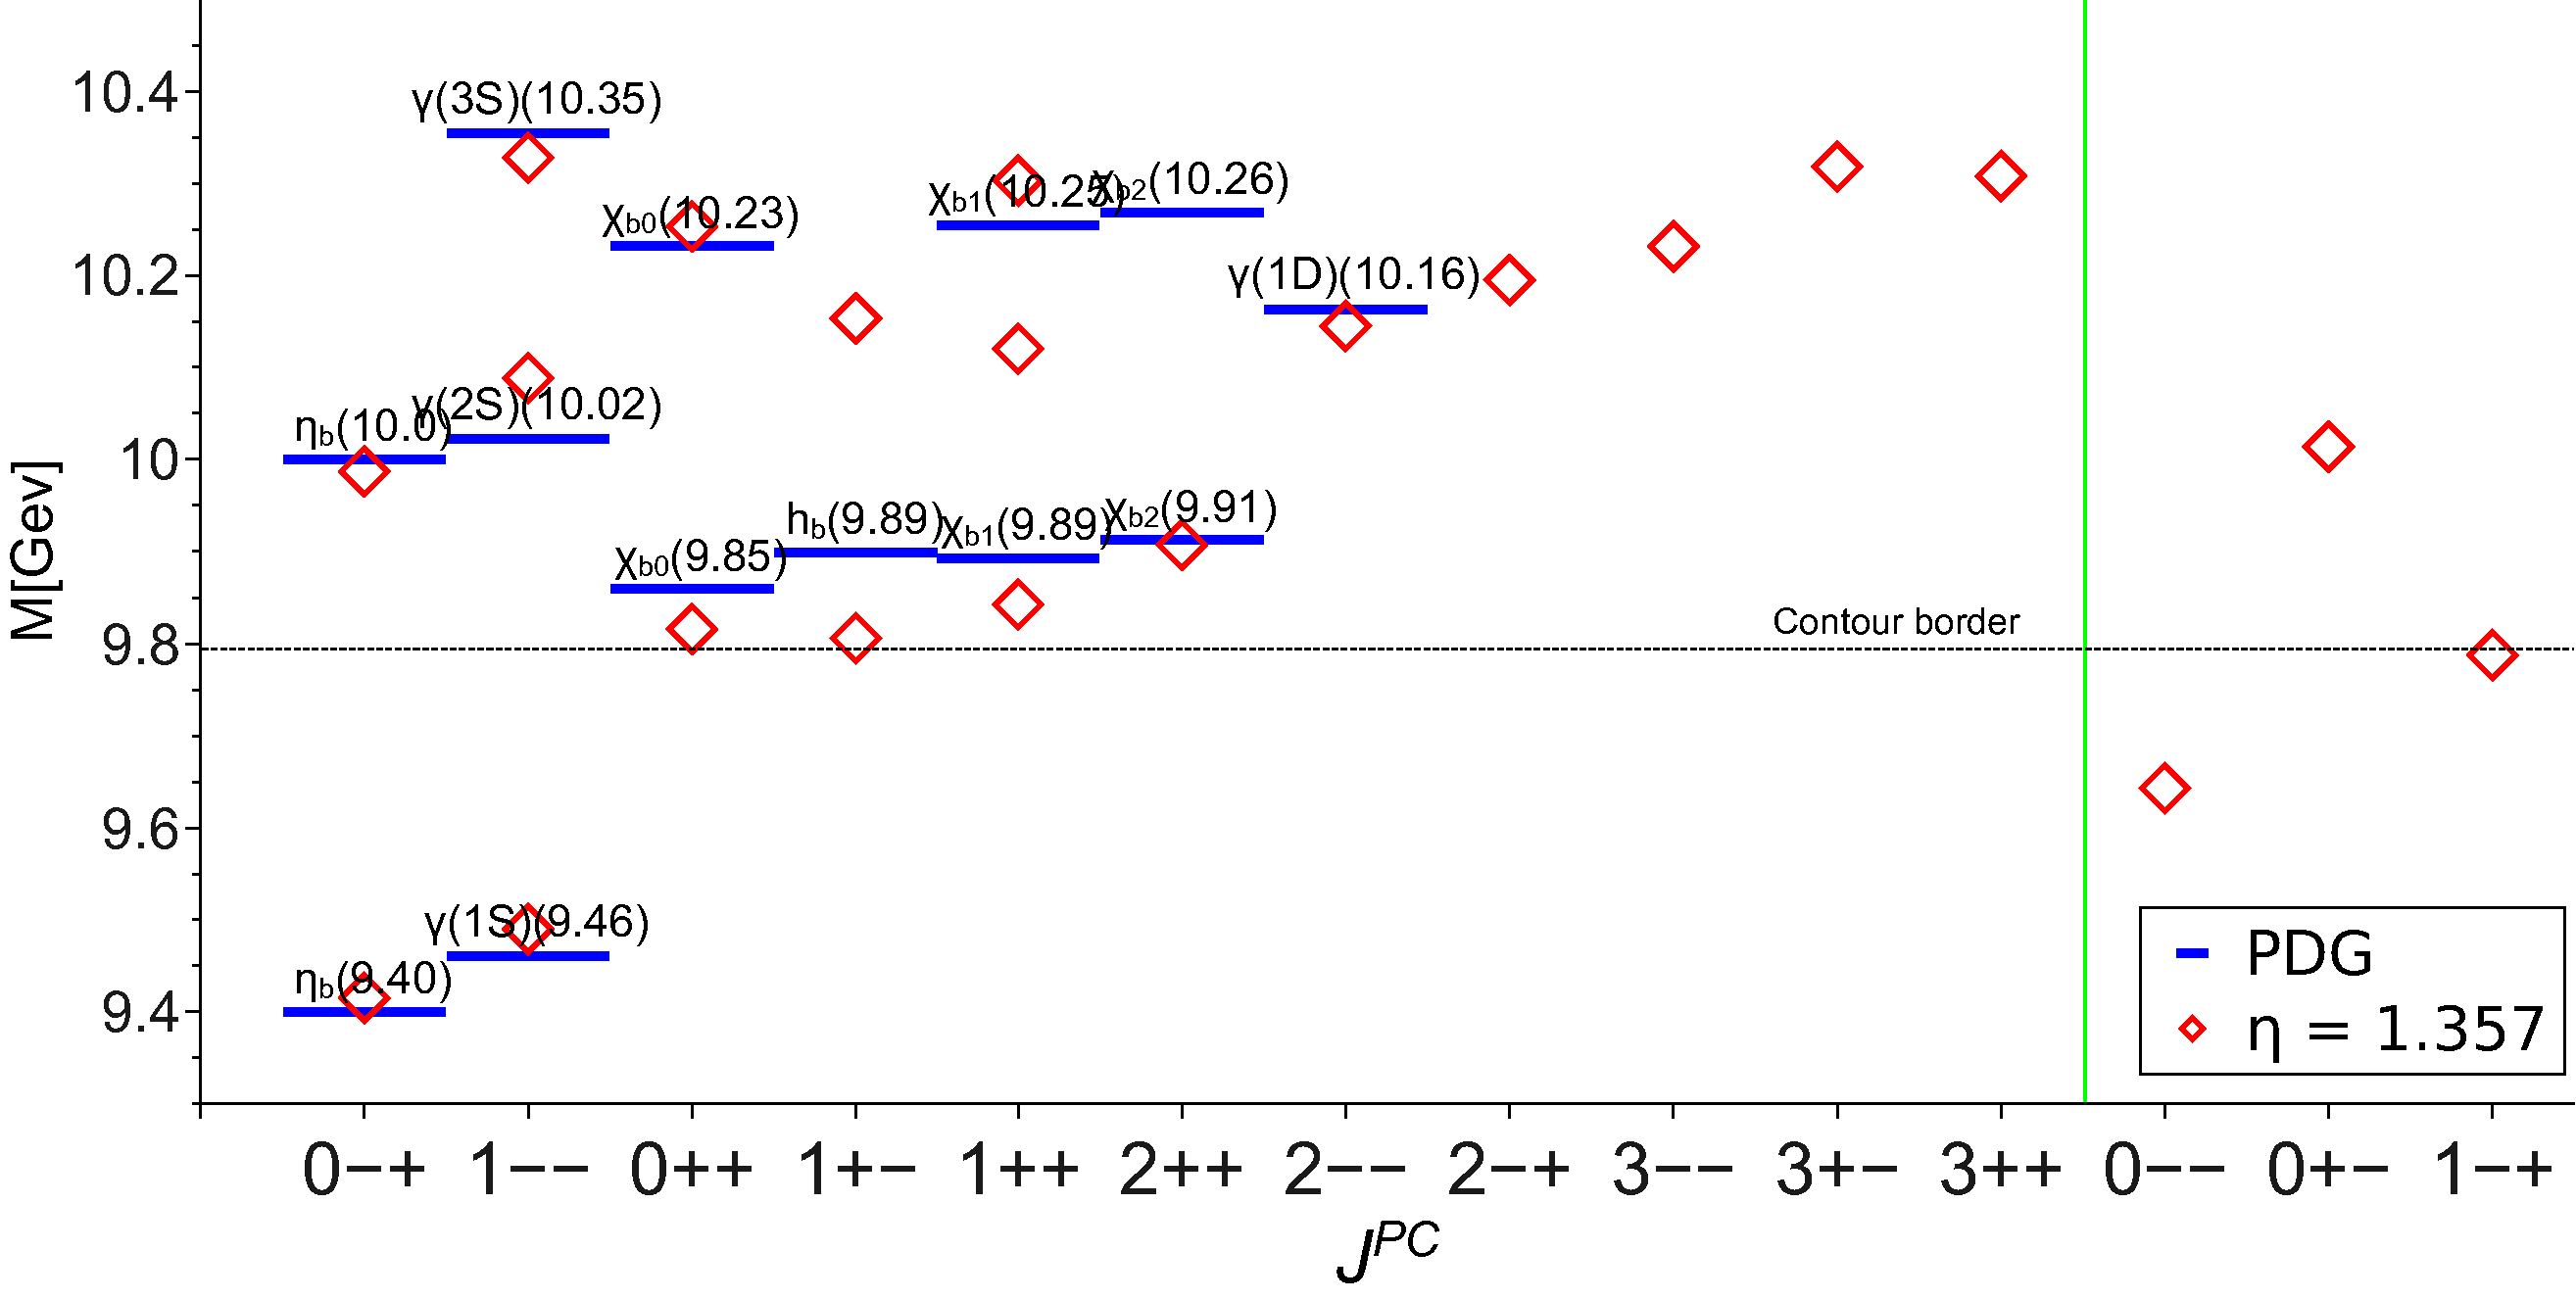
\includegraphics[width=0.999\textwidth]{figures/spectrum_bb}
    \caption{Spectrum of ground and excited bottomonium states for the vanilla MT-rainbow-ladder interaction.}\label{fig:bottom}
  \end{center}
\end{figure*}
%
In contrast to the charm-case, the lowest lying excited states in the bottomonium spectrum are
already in a mass region where we need to extrapolate the eigenvalue of the BSE, as discussed
above. Nevertheless, the extrapolation procedure seems to work and the results are surprisingly
good and comparable with the corresponding ones in the charmonium spectrum, where much less
extrapolation was needed. The first excited states in the pseudoscalar, vector and even the
scalar channel are quite accurate and even the $\Psi(3S)$ works reasonably well. In the $1^{++}$-channel
we encounter the same problem as in the charmonium spectrum, there is a first excited state 
with a much too small mass, whereas the second excited state is not too far from a PDG-state.
Again we suspect large corrections beyond rainbow-ladder in this channel.

Our results for exotic states are also given in the plot, although, as already mentioned 
for the charmonia spectrum, they should be regarded with some caution due to potential
mixing effects with non-$q\bar{q}$-states in these channels.

%
%
%
%
%

%
\begin{figure}[!thp]
  \begin{center}
    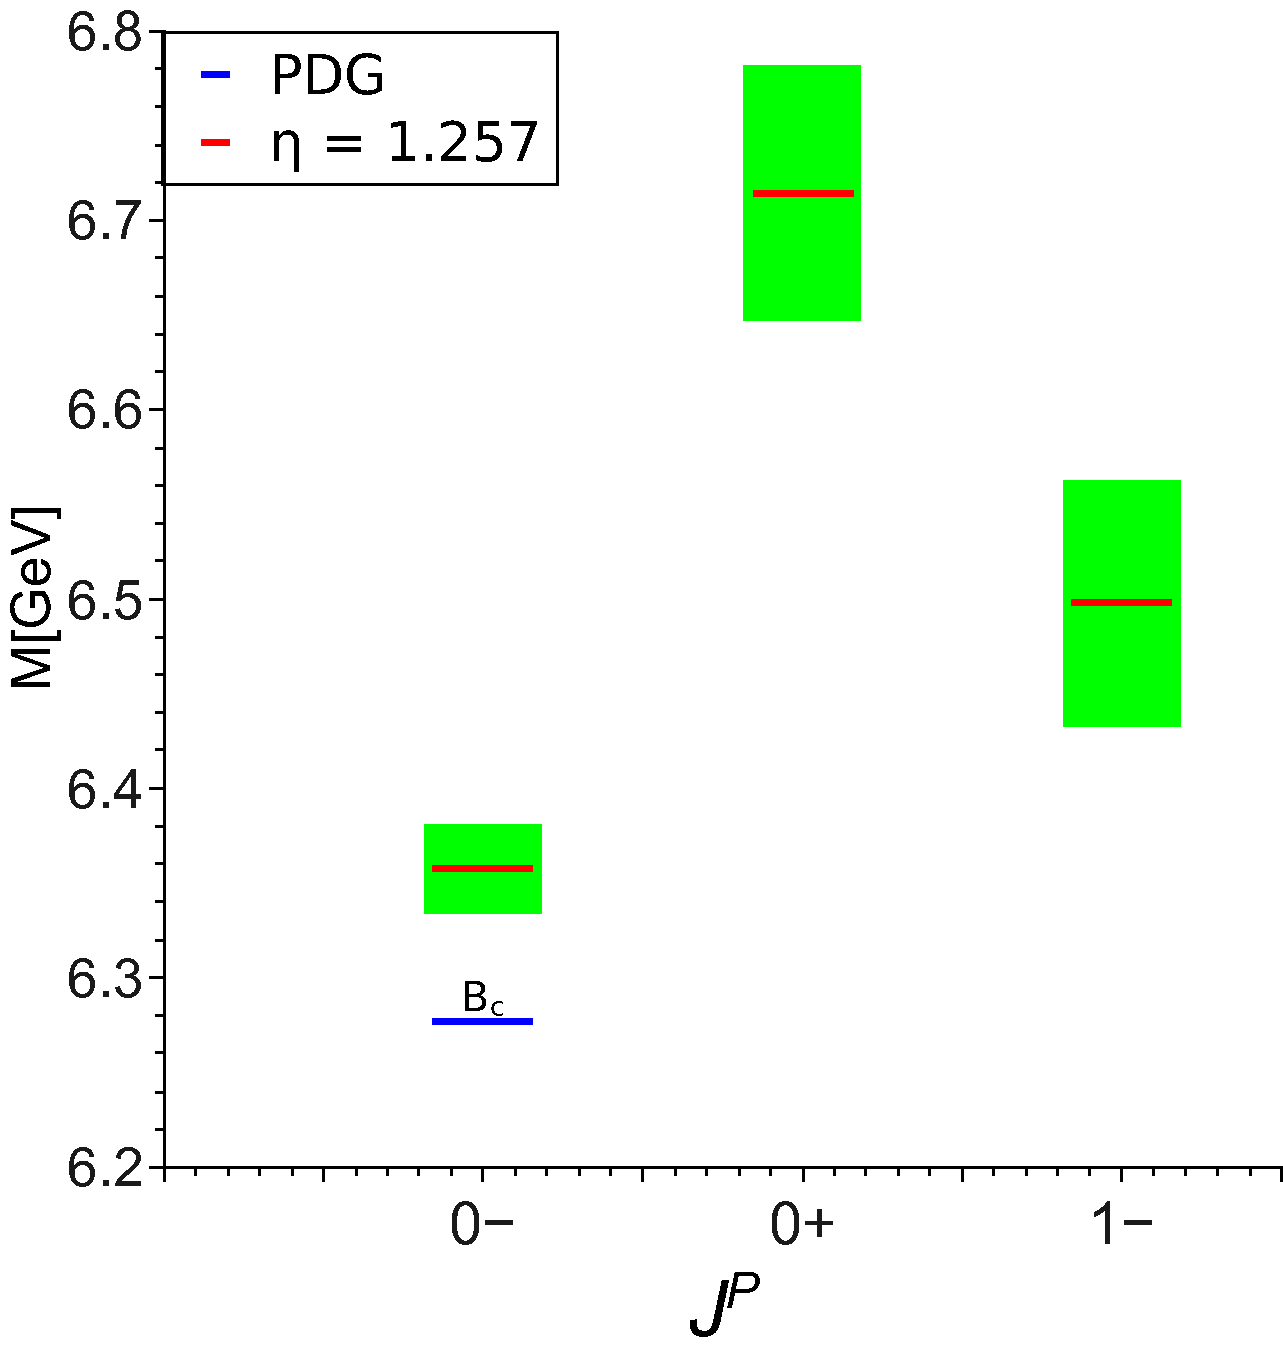
\includegraphics[width=0.45\textwidth]{figures/spectrum_bc}
    \caption{The calculated $b\bar{c}$ spectrum compared to experiment. The green bands correspond 
             to the variation $\eta=1.257\pm0.1$.}\label{fig:spectrumbc}
  \end{center}
\end{figure}

Finally, we present our results for selected channels of $B_c$-mesons. 
Heavy-light systems in the Bethe-Salpeter
approach are notoriously difficult to treat, since the problem of probing the analytical
structure of the internal quark propagators already appears for ground states, see e.g.
Ref.~\cite{Rojas:2014aka,Gomez-Rocha:2014vsa} for recent studies of the problem. Our results for these states,
shown in Fig.~\ref{fig:spectrumbc} are therefore all extrapolated and have a systematic error
of about 5-10 \%. In the plot we show values obtained using a variation of the $\eta$-parameter
in the interaction ranging approximately between the ones used for the charmonia and bottomonia.
In this way we heuristically take into account the varying strength of the interaction for the
two different quark flavours involved. The central value, given by the red line, corresponds 
to $\eta=1.257$. Given the inherent uncertainties in the calculation, our value for the $B_c$
in the pseudoscalar channel is surprisingly close to the experimental one. Since this is the
state with the lowest mass, the extrapolation error is also smallest. Since the rainbow-ladder
approach works well in the vector channel we consider the existence and to some extent also the 
mass of the vector state as a prediction of the approach, whereas the scalar channel has to
be considered with much more reservation. Despite these sources for errors it is interesting to
note that our results for all three states agree qualitatively with the ones in the relativistic 
quark model of Ref.~\cite{Ebert:2011jc} with quantitative deviations of at most 3~\%.

\begin{table*}[!t]
\renewcommand{\arraystretch}{1.3}
\begin{center}
\begin{tabular}{c|ccc|ccc||c|c}
\hline
\hline
            & \multicolumn{3}{c|}{$c\bar{c}   $}   & \multicolumn{3}{c||}{$b\bar{b}$}    & \multicolumn{2}{c}{$b\bar{c}$}                                         \\
$J^{PC}$    & $n=0$   & $n=1$  & $n=2$  & $n=0$   & $n=1$  & $n=2$  &  $J^{P}$ &    $n=0$                               \\
\hline                                                                                                                                                                                                     
$0^{-+}$    & $2925$  & $3684$ &        & $9414$  & $9987$ &    	&   $0^{+}$     &   $6714^{+67.1}_{-67.1}$           \\
$0^{--}$    & $3348$  &        &        & $9642$  &        &    	&   $0^{-}$   &     $6354^{+23.5}_{-23.5}$    \\
$0^{++}$    & $3323$  & $3833$ &        & $9815$  & $10254$&    	&  $1^{+}$   &                         \\
$0^{+-}$    & $3674$  &        &        & $10014$ &        &     	&  $1^{-}$  &     $6498^{+64.9}_{-64.9}$                                 \\
\hline                                                                                                                                                                                                     
$1^{-+}$    & $3524$  &        &        & $9788$  &        &    	&       &                 \\
$1^{--}$    & $3113$  & $3676$ & $3803$ & $9490$  & $10089$& $10327$&       &               \\ 
$1^{++}$    & $3489$  & $3672$ & $3912$ & $9842$  & $10120$& $10303$&       &               \\
$1^{+-}$    & $3433$  & $3747$ &        & $9806$  & $10154$&    	&       &                    \\
\hline                                                                                                                                                                                                     
$2^{-+}$    & $3806$  &        &        & $10194$  &        &    	&      &                                 \\
$2^{--}$    & $3739$  &        &        & $10145$  &        &    	&      &                                              \\
$2^{++}$    & $3550$  &        &        & $9906$   &        &    	&      &                                      \\
%$2^{+-}$   &         &        &        & $10194$  &        &    	&     &                                                                      \\
\hline                                                                                                                                                                                                     
%$3^{-+}$   &         &        &        &          &        &    	&      &                                        \\
$3^{--}$    & $3896$ &         &        & $10232$  &        &    	&      &                                           \\
$3^{++}$    & $3999$ &         &        & $10302$  &        &    	&       &                                     \\
$3^{+-}$    & $4037$ &         &        & $10319$  &        &    	&      &                                                   \\                                                                                                                                                                      
\hline
\hline
\end{tabular}
\caption{Calculated masses for ground and excited charmonium, bottomonium and charm-bottom states.}\label{tab:results}
\end{center}
\end{table*}

%
%
%
%
%
\subsection*{Effective interaction variation}\label{int1}
%
\begin{figure}[!t]
  \begin{center}
    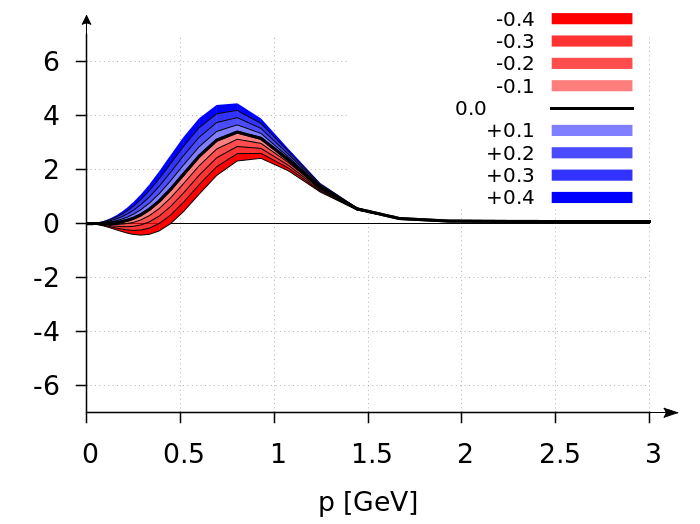
\includegraphics[width=0.38\textwidth]{figures/maris_a1}
    \caption{The shape of the effective coupling for the generalized Maris-Tandy interaction 
             with varying $a_1$ and $a_2=1$ held constant (see text for further explanations).}
    \label{fig:slope_a1}
  \end{center}
  %
  \begin{center}
    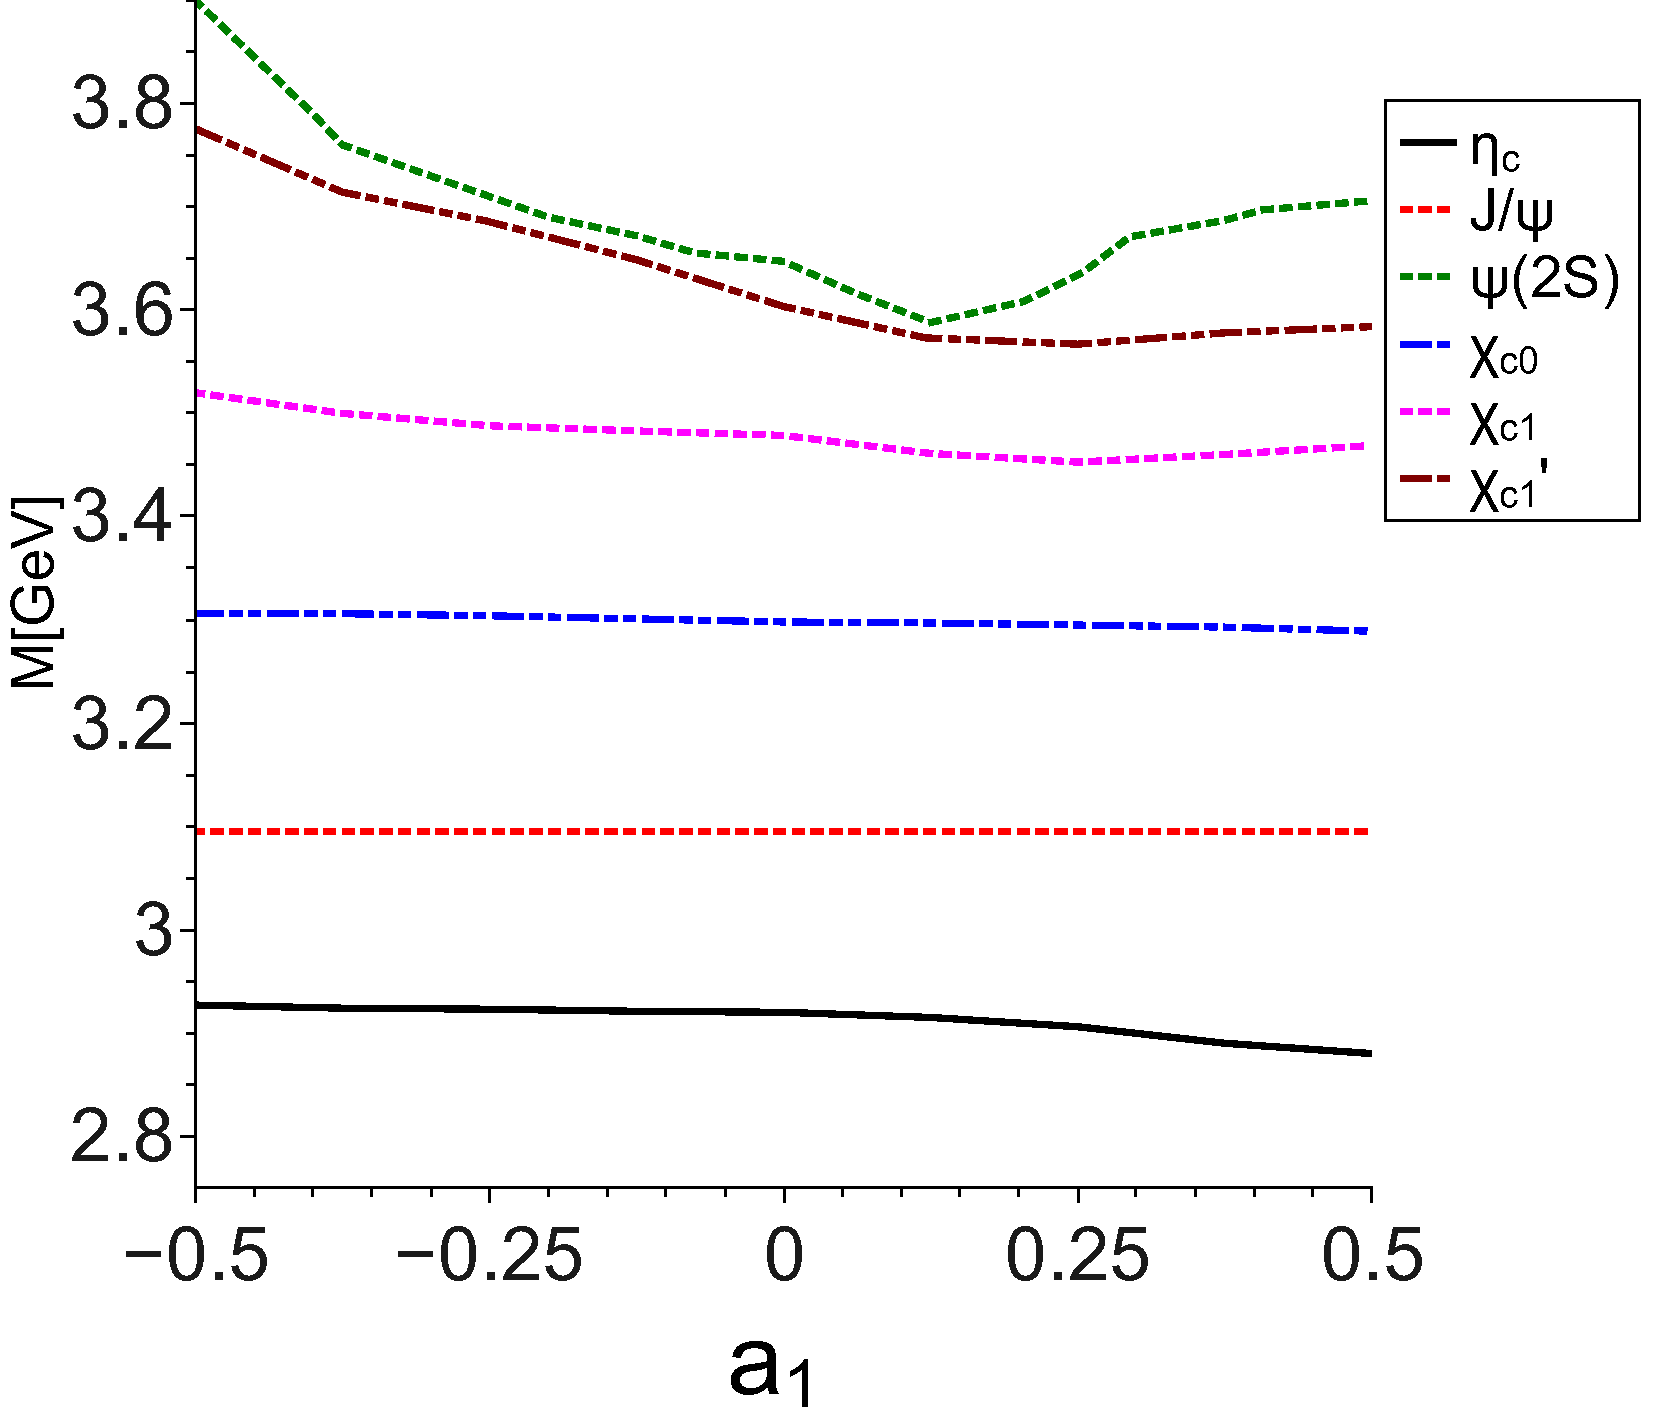
\includegraphics[scale=0.25]{figures/trend_a1_CC}
    \caption{The response of masses of bound and excited states on the variation of the shape 
             of the effective interaction with $a_1$.}
    \label{fig:trend_a1}
  \end{center}
\end{figure}
%
\begin{figure}[!t]
  \begin{center}
    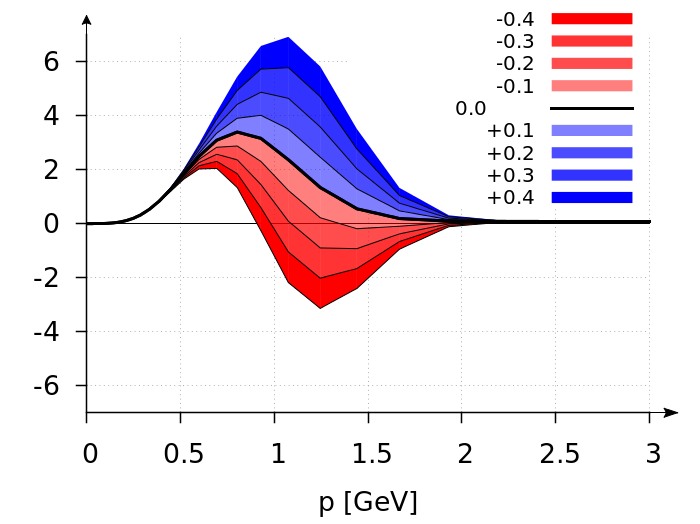
\includegraphics[width=0.38\textwidth]{figures/maris_a4}
    \caption{The shape of the running coupling for the generalized Maris-Tandy interaction with $a_2=1$, $a_1=a_3=0$ and varying $a_4$.}\label{fig:slope_a4}
  \end{center}
  %
  \begin{center}
    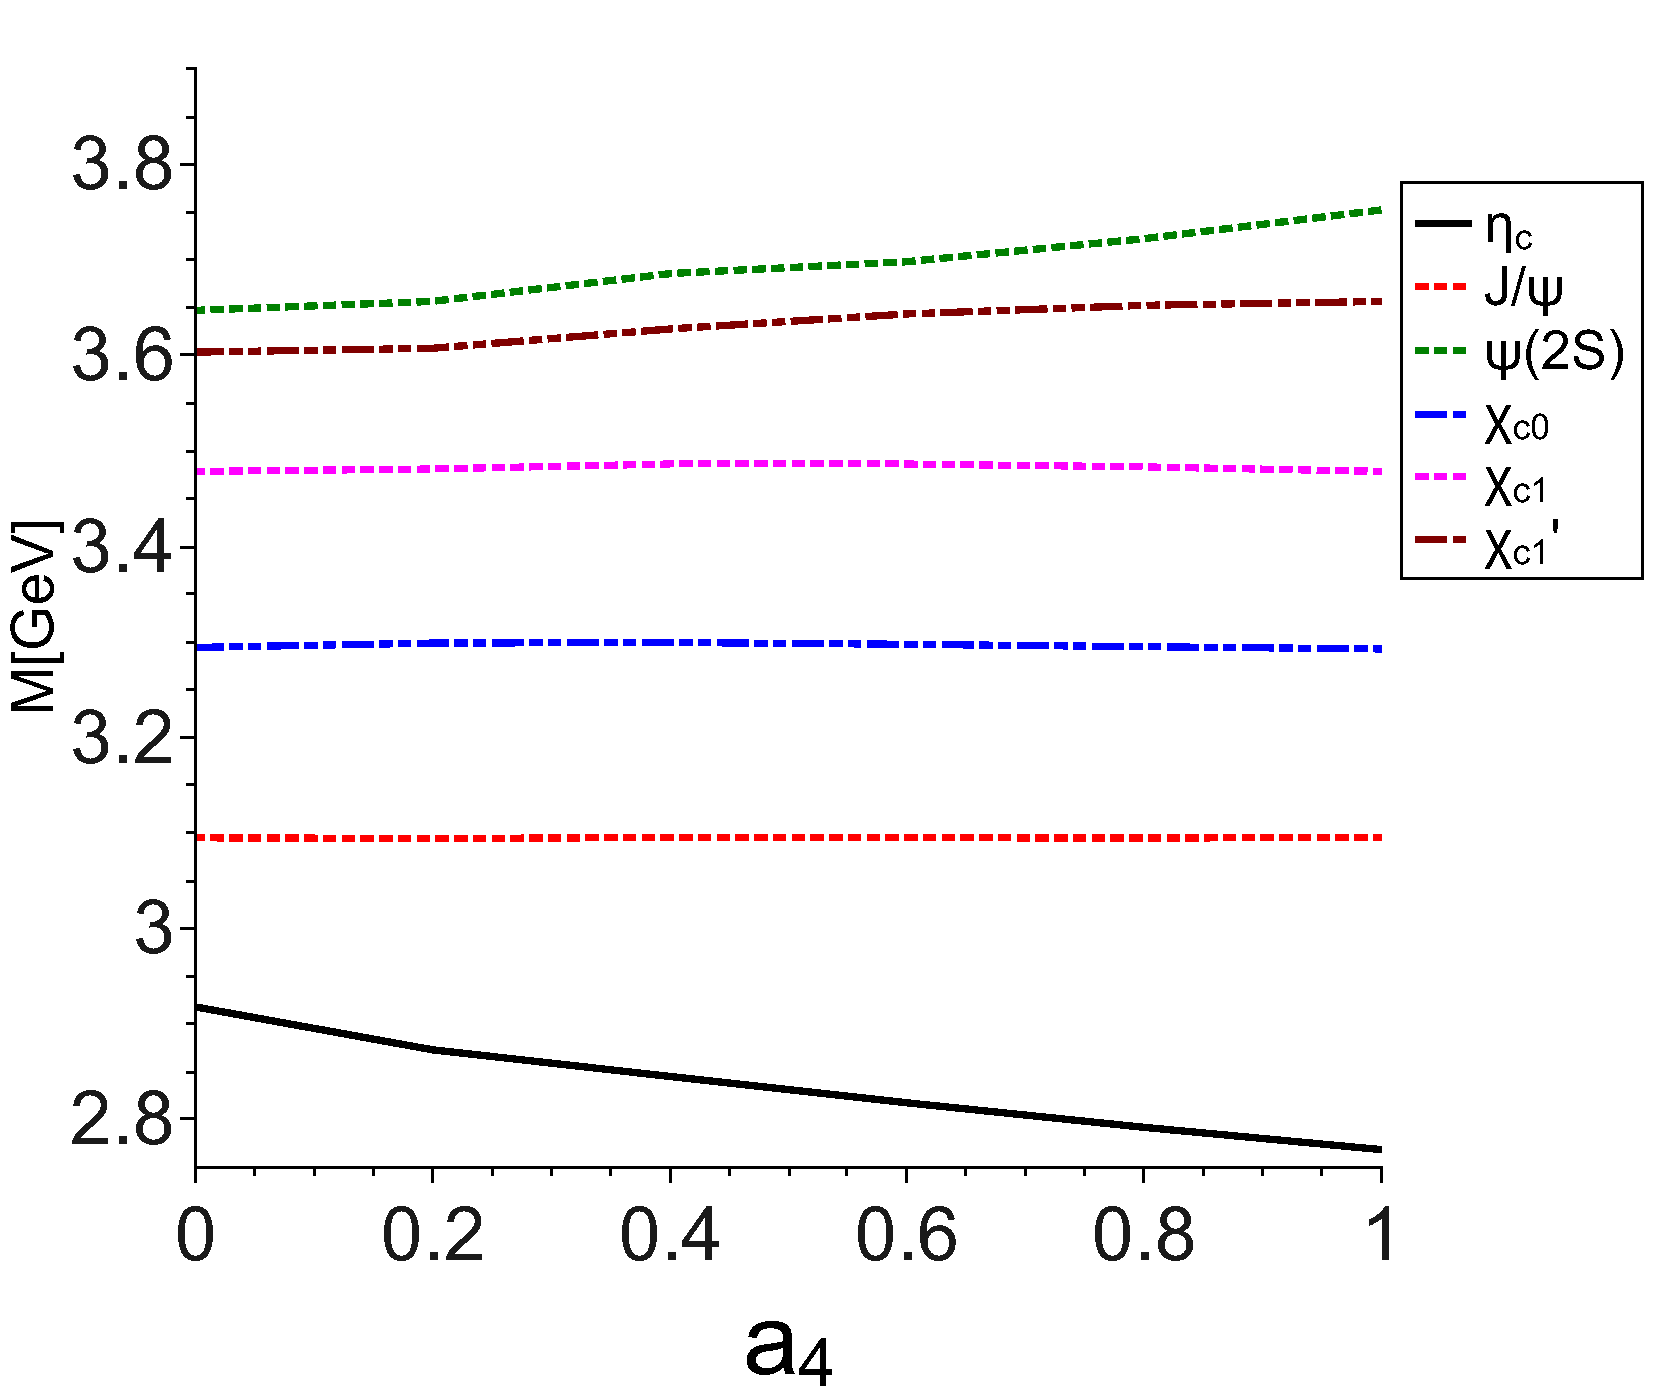
\includegraphics[scale=0.25]{figures/trend_a4_CC} 
    \caption{The response of masses of bound and excited states on the variation of the shape of the effective interaction with $a_4$.}\label{fig:trend_a4}
  \end{center}
\end{figure}

In order to study the variations of the charmonium spectrum with respect to changes in the
general momentum behaviour of the effective coupling we now introduce
additional structure in the polynomial $\mathcal{P}(x)$ in Eq.~(\ref{eqn:generalmaristandy2}). 
First we vary $a_1$ in the interval
$-0.5 \le a_1 \le 0.5$. For the effective running coupling the resulting variation
is shown in Fig.~(\ref{fig:slope_a1}). Clearly, the integrated strength, but
also the fine details of the coupling change: For negative $a_1$ we even obtain 
a zero crossing with the corresponding scale associated with the relative
strength between the $a_1$ and $a_2$-terms (here we keep $a_2=1$). Such an 
effective coupling is unusual, but not unreasonable. Recent calculations of 
the three-gluon vertex \cite{Aguilar:2013vaa,Blum:2014gna,Eichmann:2014xya} suggest that the interplay between 
ghost and gluon degrees of freedom in the corresponding Dyson-Schwinger equation 
for the vertex may very well introduce such a zero crossing. This possibility is also 
seen in corresponding lattice calculations \cite{Cucchieri:2008qm}. Since the three-gluon 
vertex is an integral part of the non-Abelian diagrams in the DSE for the quark-gluon vertex, 
this behaviour may translate into a corresponding zero crossing of the quark-gluon 
vertex~\cite{Williams:2014iea} and subsequently into the effective coupling.

The resulting changes in the meson spectrum are displayed in 
Fig.~\ref{fig:trend_a1}. Adjusting the bare charmonium quark mass via $m_{J/\Psi}$
to accommodate for the changes in the integrated interaction strength we
observe only very small changes in the resulting masses for the ground state mesons.
However, the excited states $\Psi(2S)$ and $\chi_{c1}^{\prime}$ turn out to be very sensitive 
to the details of the interaction. In particular for negative values of $a_1$,
corresponding to the zero crossing of the interaction discussed above, we find much
increased values for the mass of the $\chi_{c1}^{\prime}$, which eventually even may 
hit the experimentally observed mass of the $X(3872)$. However, this comes at a price: 
the mass of the $\Psi(2S)$ reacts in a similar way and substantially moves away from 
the experimental value, almost reproduced for $a_1=0$. We therefore conclude, that 
by changing the infrared behaviour of our rainbow-ladder interaction it is not possible 
to accommodate for the quark-antiquark nature of the $X(3872)$, while at the same time 
keeping the remaining spectrum intact.


%
%
%
%
%

Next we consider the generalized Maris-Tandy interaction, Eq.~(\ref{eqn:generalmaristandy2}), 
given by $a_1=0$, $a_2=1$ but non-trivial components $a_3$ or $a_4$. Both of these modify 
the interaction in the intermediate momentum region, while keeping the infrared and
ultraviolet behaviour untouched as can be seen from Fig.~\ref{fig:slope_a4} for the 
example of variations in $a_4$. Since variations of $a_3$ act similarly on the effective
coupling we keep $a_3=0$ fixed and restrict ourselves to variations of $a_4$.
Furthermore, we keep $a_4 \ge 0$, since there are no indications that the dressing of the
quark-gluon vertex can induce a negative effective interaction in the mid-momentum region
(in contrast to the infrared momentum region discussed in section \ref{int1} above).

Again, we study the variation of the charmonium spectrum while still readjusting
the charm quark mass to reproduce the vector ground state $J/\Psi$. Our results
are given in Fig.~\ref{fig:trend_a4}. Here we find a substantial increase in the
mass splitting between the pseudoscalar and the vector channel due to the additional
interaction strength in the mid-momentum region. At the same time, the masses of the
excited state, $\Psi(2S)$ and $\chi_{c1}^{\prime}$ increase slightly. This moderate increase 
is nowhere large enough to bring the $\chi_{c1}^{\prime}$ close to the observed $X(3872)$-state.
Thus we arrive at the conclusion that by changing the mid-momentum behaviour of our 
interaction it is not possible to accommodate for a quark-antiquark nature of the 
$X(3872)$, while at the same time keeping the remaining spectrum intact.
%
%
%
%
%
%%
%
%
%
%

In this work we presented a first calculation of ground and excited states with angular 
momentum $J \le 3$ in the heavy quark sector using the framework of Dyson-Schwinger 
and Bethe-Salpeter equations. We have used a simple interaction model, the rainbow-ladder
approximation, which is known to represent only part of the complicated interaction
pattern of quarks and gluons even for heavy quarks. Nevertheless, we obtained surprisingly 
good results, at least for selected quantum numbers. In general, the systematics in the 
spectrum for charmonia and bottomonia is very similar, although the underlying interaction 
is not the same. Compared to the light quark sector, where
the rainbow-ladder approximation has clear deficiencies \cite{Fischer:2014xha}, the agreement with
the experimental states is much improved. This is particularly true for the ground and 
excited charmonia and bottomonia states in the vector channel, where even the second 
radial excitation is well represented. For pseudoscalar states and tensor states with quantum 
number $2^{++}$ we obtain reasonable results, whereas for scalars and axialvectors some
deviations occur. We also gave predictions for the other tensor states, in particular
for the $3^{--}$, which should be a channel where the rainbow-ladder approximation
does particularly well. For the bottomonia, our values for the tensor states may be 
considered as solid predictions for experiment with a systematic error due to 
extrapolations on the 1~\% level. We also gave results for $B_c$ states and quarkonia 
with exotic quantum numbers, although the accumulated errors in these channels due to
deficiencies in the rainbow-ladder interaction may be sizeable.

Furthermore, we studied variations of the shape of the rainbow-ladder effective coupling with 
the aim to explore whether the first excitation in the $1^{++}$-channel can be linked 
to the $X(3872)$ without destroying other parts of the spectrum. It turned out, that 
this is not possible. Thus either hitherto not included corrections beyond rainbow-ladder
play an important role in this channel, or the $X(3872)$ does indeed not have a strong
quark-antiquark component. From the perspective of our framework, these questions remain 
open until studies beyond rainbow-ladder are available. 

Clearly, the findings of this work should be corroborated by studies beyond the 
simple rainbow-ladder scheme used in this work. Within the light meson sector
several approaches in this direction have been explored in the past 
\cite{Watson:2004kd,Fischer:2005en,Fischer:2008wy,Fischer:2009jm,Chang:2009zb,Heupel:2014ina}
and it remains to be seen whether these can be transferred to the heavy quark 
sector. This will the subject of future work.
	
	